%This document includes programs with version numbers (e.g. cgg, boost).
%They need to be updates, when the programs are.
%These appear on the following sections:

%Obtaining Kaskade7 and third-party software (section 3.1, pages 13-15): Kaskade;
%Compiler and Libraries (section 3.3, page 16): alberta, boost, gcc;
%External libraries (section 4, pages 20-23): alberta, alugrid, boost, Dune, hypre, Mumps, superlu, taucs, umfpack
%Linear solver (section 9.1, page 67): Mumps, Pardiso, umfpack, superlu


%!TEX encoding = UTF-8 Unicode
%!TEX TS-program = pdflatex
%\documentclass{svmult}
\documentclass[11pt]{article}

%\usepackage[T1]{fontenc}
%\usepackage[latin1]{inputenc}
%\usepackage{color}
%\usepackage{geometry}\geometry{a4paper}
%\usepackage[parfill]{parskip}
%\usepackage{graphicx}
%\usepackage{amssymb}
%\usepackage{epstopdf}
%\usepackage{datetime}
%\usepackage[colorlinks,urlcolor=blue,citecolor=red]{hyperref}
%\usepackage{fancyvrb}
%\usepackage{url}
%\usepackage{natbib}

% spaces after macros but not when . or , or something is following
\usepackage{xspace}
\usepackage{listings}
\lstset{language=C++,basicstyle=\ttfamily}

% dune core modules 
\newcommand{\dune}{\textsc{Dune}\xspace}
\newcommand{\dunecommon}{\textsc{Dune-Common}\xspace}
\newcommand{\dunegrid}{\textsc{Dune-Grid}\xspace}
\newcommand{\duneistl}{\textsc{Dune-Istl}\xspace}
\newcommand{\dunelocalfunctions}{\textsc{Dune-Localfunctions}\xspace}

% external modules 
\newcommand{\dunefem}{\textsc{Dune-Fem}\xspace}
\newcommand{\dunepdelab}{\textsc{Dune-PDELab}\xspace}
\newcommand{\dumux}{\textsc{DuMu}$^\textrm{x}$\xspace}

% external packages
\newcommand{\alugrid}{\textsc{ALUGrid}\xspace}
\newcommand{\alberta}{\textsc{ALBERTA}\xspace}

% grid names 
\newcommand{\albertagrid}{{\tt AlbertaGrid}\xspace}
\newcommand{\alusimplexgrid}{{\tt ALUSimplexGrid}\xspace}
\newcommand{\alucubegrid}{{\tt ALUCubeGrid}\xspace}
\newcommand{\aluconformgrid}{{\tt ALUConformGrid}\xspace}
\newcommand{\uggrid}{{\tt UGGrid}\xspace}
\newcommand{\onedgrid}{{\tt OneDGrid}\xspace}
\newcommand{\sgrid}{{\tt SGrid}\xspace}
\newcommand{\yaspgrid}{{\tt YaspGrid}\xspace}



%% Proceedings styles
\usepackage{mathptmx,helvet,courier,multicol}
\usepackage[bottom]{footmisc}
\usepackage{color}
\usepackage{listings}
%\lstset{language=C++,basicstyle=\ttfamily\small,breaklines=true}
%%------------------SG:added---------------------------------------------------------------
\definecolor{listinggray}{gray}{0.9}
\definecolor{lbcolor}{rgb}{0.9,0.9,0.9}
% \lstset{
% backgroundcolor=\color{lbcolor},
%    tabsize=4,    
%   rulecolor=,
%    language=[GNU]C++,
%        basicstyle=\scriptsize,
%        upquote=true,
%        aboveskip={1.5\baselineskip},
%        columns=fixed,
%        showstringspaces=false,
%        extendedchars=false,
%        breaklines=true,
%        prebreak = \raisebox{0ex}[0ex][0ex]{\ensuremath{\hookleftarrow}},
%        frame=single,
%        %numbers=left,
%        showtabs=false,
%        showspaces=false,
%        showstringspaces=false,
%        identifierstyle=\ttfamily,
%        keywordstyle=\color[rgb]{0,0,1},
%        commentstyle=\color[rgb]{0.026,0.112,0.095},
%        stringstyle=\color[rgb]{0.627,0.126,0.941},
%        numberstyle=\color[rgb]{0.205, 0.142, 0.73},
%        \lstdefinestyle{C++}{language=C++,style=numbers}’.
% }
\lstset{
    backgroundcolor=\color{lbcolor},
    tabsize=2,
  language=C++,
  captionpos=b,
  tabsize=3,
  frame=lines,
  %numbers=left,
  %numberstyle=\tiny,
  numbersep=5pt,
  breaklines=true,
  showstringspaces=false,
  basicstyle=\footnotesize,
%  identifierstyle=\color{magenta},
  keywordstyle=\color[rgb]{0,0,1},
  commentstyle=\color[rgb]{0,0.6,0}, %darkgreen
  stringstyle=\color{red}
  }
%%---------------------------------------------SG:remove-------------------------------------------------
%%
%% Packages to be used.
%%
\usepackage[utf8]{inputenc}
\usepackage{amsmath,amsfonts}
\usepackage{booktabs}
\usepackage{vruler}
\usepackage{fancyvrb}

%%
%% PDF / DVI output
%%
\usepackage[pdftex]{graphicx}
\usepackage[pdftex]{thumbpdf}
\usepackage{epstopdf}
\usepackage{url}
\usepackage{hyperref}

%%
%% Special sets.
%%
\newcommand{\N}{\mathbb{N}}
\newcommand{\R}{\mathbb{R}}
\newcommand{\One}{\boldsymbol{1}}

%%
%% Mathematical convenience.
%%
%\DeclareMathOperator{\ld}{ld}
%\DeclareMathOperator{\convex}{co}
%\newcommand{\half}{\frac{1}{2}}
\newcommand{\Ol}[1]{\mathcal{O}(#1)}
\newcommand{\dual}[1]{#1^\star}
\newcommand{\norm}[1]{\left\|#1\right\|}
\newcommand{\const}{\mathrm{const}\,}

\newcommand{\autoptr}{{\tt std::auto\_ptr}}
\newcommand{\uniqueptr}{{\tt std::unique\_ptr}}
\newcommand{\fusionvector}{{\tt boost::fusion::vector}}

\newcommand{\K}{\textsc{Kaskade7 }}

\newcommand{\boost}[1]{\textsc{boost#1}}


\usepackage{makeidx}

\makeindex

\title{\K Finite Element Toolbox \\ {\em Programmers Manual} }
%\title{\includegraphics[scale=0.36]{RTEmagicC_68b9c7c75f.png} \vspace{4mm}Finite Element Toolbox \\ {\em Programmers Manual} }
\author{M.~Weiser, A.~Schiela, S.~G\"otschel, L.~Lubkoll \\B.~Erdmann, L.~Weimann, M.~Moldenhauer, F.~Lehmann, J.~Schneck} \date{\today}

%%%%%%%%%%%%%%%%%%%%%%%%%%%%%%%%%%%%%%%%%%%%%%%%%%%%%%%%%%%%%%%%%%%%%%%%%
\begin{document}


\maketitle
\vspace{8cm}
%\centerline{\includegraphics[scale=0.36]{K7logo.png}}
\centerline{\includegraphics[scale=0.36]{../../doc/logo/kaskade.png}}

\newpage
\tableofcontents
\newpage

\pagestyle{myheadings}
\thispagestyle{plain}

\section{Introduction} \index{Kaskade~7} \label{intro}
\K is a general-purpose finite element toolbox for solving systems of elliptic and parabolic PDEs. Design targets for the \K code have been \emph{flexibility}, \emph{efficiency}, and \emph{correctness}.   One possibility to achieve these, to some extent competing, goals is to use C++ with a great deal of template metaprogramming~\cite{Veldhuizen1995}. This generative programming technique uses the C++ template system to let the compiler perform code generation. The resulting code is, due to static polymorphism, at the same time type and const correct and, due to code generation, adapted to the problem to be solved. Since all information relevant to  code optimization is directly available to the compiler, the resulting code is highly efficient, of course depending on the capabilities of the compiler. In contrast to explicit code generation, as used, e.g., by the \textsc{FEniCS} project~\cite{Logg2007}, no external toolchain besides the C++ compiler/linker is required. Drawbacks of the template 
metaprogramming approach are longer compile times, somewhat cumbersome template notation, and hard to digest compiler diagnostics. Therefore, code on higher abstraction levels, where the performance gains of inlining and avoiding virtual function calls are negligible, uses dynamic polymorphism as well.

The \K code is heavily based on the \dune \index{Dune} libraries~\cite{BastianBlattDednerEngwerKloefkornOhlbergerSander2008,BastianBlattDednerEngwerKloefkornKornhuberOhlbergerSander2008,BlattBastian2007,dune}, which are used in particular for grid management, numerical quadrature, and linear algebra.


In Section \ref{design} we describe the design and structure of \K, also presenting some details of the implementation.
The next section presents more practical advices to use the code. In particular, we give hints how to install the code and
a set of third-party software needed in \K. 

Following the guideline of the sections \ref{Install}, \ref{libs}, and \ref{docu}
the user can provide all the technical requirements necessary to start his/her own programming. 
This should be accompanied by the tutorial including a set of examples in Section \ref{examples}.

Subsequent to that {\em Getting started} chapter we bring more and more details about programming
of certain classes and modules helping the user of \K to extend his knowledge and get familiar to
all the topics interesting for developers. We close with a gallery of projects dealt with \K, some notes
on the history of development of the code, and finally a list of publications using simulation results
provided by \K.


\section{Structure and Implementation} \label{design}

As a guiding example at which to illustrate features of \K we will use in this section the all-at-once approach to the following simple optimal control problem.\index{optimal control problem! elliptic} 
For a desired state $y_d$ defined over a domain $\Omega\subset \R^d$, $d\in\{1,2,3\}$, and $\alpha>0$ we consider the tracking type problem
\[
  \min_{u\in L^2(\Omega), y\in H^1_0(\Omega)} \frac{1}{2}\|y-y_d\|_{L^2(\Omega)}^2 + \frac{\alpha}{2} \|u\|_{L^2(\Omega)}^2 \quad\text{s.t.}\quad -\Delta y = u \quad\text{in $\Omega$}.
\]
The solution is characterized by the Lagrange multiplier $\lambda\in H^1_0(\Omega)$ satisfying the Karush-Kuhn-Tucker system
\[
  \begin{bmatrix}
    I & & \Delta \\ & \alpha & I \\ \Delta & I &
  \end{bmatrix}
  \begin{bmatrix}
    y \\ u \\ \lambda
  \end{bmatrix}
  =
  \begin{bmatrix}
    y_d \\ 0 \\ 0
  \end{bmatrix}.
\]

For illustration purposes, we will discretize the system using piecewise polynomial finite elements for $y$ and $\lambda$ and piecewise constant functions for $u$, even though this is not the best way to approach this particular type of problems~\cite{HinzeEtAl09,WeiserGaenzlerSchiela2008}.

The foundation of all finite element computation is the approximation of solutions in finite dimensional function spaces. In this section, we will discuss the representation of functions in \K before addressing the problem formulation.

\subsection{Finite Element Spaces} \label{FEspaces}
On each reference element $T_0$ there is a set of possibly vector-valued shape functions $\phi_i:T_0\to \R^s$, $i=1,\dots,m$ defined. Finite element functions are built from these shape functions by linear combination and transformation. More precisely, finite element functions defined by their coefficient vectors $a\in\R^N$ are given as
\[
  u(x)|_T = \psi_T(x)(\Phi(\xi)K_Ta_{I_T}) ,
\]
where $a_{I_T}\in \R^k$ is the subvector of $a$ containing the coefficients of all finite element ansatz functions which do not vanish on the element $T$, $K\in\R^{m\times k}$ is a matrix describing the linear combination of shape functions $\phi_i$ to ansatz functions $\varphi_j$, $\Phi(\xi)\in\R^{s\times m}$ is the matrix consisting of the shape functions' values at the reference coordinate $\xi$ corresponding to the global coordinate $x$ as columns, and $\psi_T(x)\in\R^{s\times s}$ is a linear transformation from the values on the reference element to the actual element $T$.

The indices $I_T$ and efficient application of the matrices $K_T$ and $\psi_T(x)$ are provided by local-to-global-mappers, in terms of which the finite element spaces are defined. The mappers do also provide references to the suitable shape function set, which is, however, defined independently. For the computation of the index set $I_T$ the mappers rely on the \dune index sets provided by the grid views on which the function spaces are defined.

For Lagrange ansatz functions, the combiner  $K$ is just a permutation matrix, and the converter $\psi(x)$ is just 1. For hierarchical ansatz functions in 2D and 3D, nontrivial linear combinations of shape functions are necessary. The implemented over-complete hierarchical FE spaces require just signed permutation matrices~\cite{Zumbusch1995}. Vectorial ansatz functions, e.g. edge elements, require nontrivial converters $\psi(x)$ depending on the transformation from reference element to actual element. The structure in principle allows to use heterogeneous meshes with different element topology, but the currently implemented mappers require homogeneous meshes of either simplicial or quadrilateral type.


In \K, finite element spaces are template classes parameterized with a mapper, defining the type of corresponding finite element functions and supporting their evaluation as well as prolongation during grid refinement, see Sec.~\ref{subsec:adaptivity}. Assuming that {\tt View} is a suitable \dune grid view type, FE spaces for the guiding example can be defined as:

%\begin{scriptsize}
%\begin{verbatim}
\begin{lstlisting}
using H1Space = FEFunctionSpace<ContinuousLagrangeMapper<double,View>>;
using L2Space = FEFunctionSpace<DiscontinuousLagrangeMapper<double,View>>;
H1Space h1Space(gridManager,view,order);
L2Space l2Space(gridManager,view,0);
\end{lstlisting}
%\end{verbatim}
%\end{scriptsize}
The type aliases for common FE spaces as above are predefined in \texttt{fem/spaces.hh} for convenience. They are parametrized over the grid type (and scalar type, with double as default). The space definition above could thus be written as follows.
\begin{lstlisting}
#include "fem/spaces.hh"
...
H1Space<Grid> h1Space(gridManager,view,order);
L2Space<Grid> l2Space(gridManager,view,0);
\end{lstlisting}


Multi-component FE functions are supported, which gives the possibility to have vector-valued variables defined in terms of 
scalar shape functions. E.g., displacements in elastomechanics and temperatures in the heat equation share the same FE space. 
FE functions as elements of a FE space can be constructed using the type provided by that space:

%\begin{scriptsize}
%\begin{verbatim}
\begin{lstlisting}
H1Space::Element<1>::type y(h1Space), lambda(h1Space);
L2Space::Element<1>::type u(l2Space);
\end{lstlisting}
%\end{verbatim}
%\end{scriptsize}

\noindent FE functions provide a limited set of linear algebra operations. Having different types for different numbers of components detects the mixing of incompatible operands at compile time.

During assembly, the ansatz functions have to be evaluated repeatedly. In order not to do this separately for each involved FE function, FE spaces define {\tt Evaluators} doing this once for each involved space. When several FE functions need to be evaluated at a certain point, the evaluator caches the ansatz functions' values and gradients, such that the remaining work is just a small scalar product for each FE function.

\subsection{Problem Formulation} \label{problemDef}
For stationary variational problems, the \K core addresses variational functionals of the type

\begin{equation}\label{basicvariational}
  \min_{u_i\in V_i} \int_{\Omega} F(x,u_1,\dots,u_n,\nabla u_1,\dots,\nabla u_n) \, dx + \int_{\partial \Omega} G(x,u_1,\dots,u_n) \,ds.
\end{equation}
In general, this problem is nonlinear. Therefore we formulate the Newton iteration in order to find the solution $u = (u_1, \dots, u_n)^T$:

Starting with an initial guess $u^0$ for $u$ we compute the Newton update  $\delta u$ by

\begin{equation}\label{newtonUpdate}
  \int_{\Omega} F''(u^0)[\delta u,v] \, dx + \int_{\partial \Omega} G''(u^0)[\delta u,v] \, ds = 
  -\int_{\Omega} F'(u^0) v \,dx - \int_{\partial \Omega} G'(u^0) v \,ds \quad \forall v \in V
\end{equation}
The approximation after one step is
\[
u_{new} = u^0 + \delta u.
\]


\noindent The problem definition consists of providing $F$, $G$, and their first and second directional derivatives in a certain 
fashion. First, the number of variables, their number of components, and the FE space they belong to have to be specified. 
This partially static information is stored in heterogeneous, statically polymorphic containers from 
the \textsc{Boost Fusion}~\cite{boost} library. Variable descriptions are parameterized over 
their space index in the associated container of FE spaces, their number of components, and their unique, contiguous id in arbitrary order.

%\begin{scriptsize}
%\begin{verbatim}
\begin{lstlisting}
typedef boost::fusion::vector<H1Space*,L2Space*> Spaces;
Spaces spaces(&h1Space,&l2Space);
typedef boost::fusion::vector<
           Variable<SpaceIndex<0>,Components<1>,VariableId<0> >, 
           Variable<SpaceIndex<0>,Components<1>,VariableId<1> >, 
           Variable<SpaceIndex<1>,Components<1>,VariableId<2> > > VarDesc;
\end{lstlisting}
%\end{verbatim}
%\end{scriptsize}


\noindent Besides this data, a problem class defines, apart from some static meta information, two mandatory member classes, the 
{\tt DomainCache} defining $F$ and the {\tt BoundaryCache} defining $G$. The domain cache provides member 
functions {\tt d0}, {\tt d1}, and {\tt d2} evaluating $F(\cdot)$, $F'(\cdot)v_i$, and $F''(\cdot)[v_i,w_j]$, 
respectively. For the  guiding example with

\[
  F = \frac{1}{2}(y-y_d)^2 + \frac{\alpha}{2}u^2 + \nabla\lambda^T \nabla y - \lambda u,
\]

\noindent the corresponding code looks like

\begin{lstlisting}
  double d0() const {
    return (y-yd)*(y-yd)/2 + u*u*alpha/2 + dlambda*dy - lambda*u;
  }
  template <int i, int d>
  double d1(VariationalArg<double,d> const& vi) const {
    if (i==0) return (y-yd)*vi.value + dlambda*vi.derivative;
    if (i==1) return alpha*u*vi.value - lambda*vi.value;
    if (i==2) return dy*vi.derivative - u*vi.value;
  }
  template <int i, int j, int d>
  double d2(VariationalArg<double,d> const& vi,
            VariationalArg<double,d> const& wj) const {
    if (i==0 && j==0) return vi.value*wj.value;
    if (i==0 && j==2) return vi.derivative*wj.derivative;
    if (i==1 && j==1) return alpha*vi.value*wj.value;
    if (i==1 && j==2) return -vi.value*wj.value;
    if (i==2 && j==0) return vi.derivative*wj.derivative;
    if (i==2 && j==1) return -vi.value*wj.value;
  }
\end{lstlisting}

\noindent A static member template class \verb?D2? defines which Hessian blocks are available. Symmetry is auto-detected, such that in \verb?d2? only $j\le i$ needs to be defined.
\begin{lstlisting}
  template <int row, int col>
  class D2 {
    static int present = (row==2) || (row==col);
  };
\end{lstlisting}

\noindent The boundary cache is defined analogously.

The functions for $y$, $u$, and $\lambda$ are specified (for nonlinear or instationary problems in form of FE functions) on construction of the caches, and can be evaluated for each quadrature point using the appropriate one among the evaluators provided by the assembler:
\begin{lstlisting}
  template <class Pos, class Evaluators>
  void evaluateAt(Pos const& x, Evaluators const& evaluators) {
      y = yFunc.value(at_c<0>(evaluators));
      u = uFunc.value(at_c<1>(evaluators));
      lambda = lambdaFunc.value(at_c<0>(evaluators));
      dy = yFunc.derivative(at_c<0>(evaluators));
      dlambda = lambdaFunc.derivative(at_c<0>(evaluators));
  }
\end{lstlisting}

\paragraph{Hint.} Usage of \verb|at_c<int>|

The function \verb|at_c<int>()| allows one to access the elements of a
heterogeneous array, that is an array, with possibly different data
types (as opposed to the \verb|std::array|, where the data type is fixed
at initialisation to one type). An example for this is above in the method \verb|evaluateAt()|. The data
type \verb|evaluators| contains evaluators of different type for the continuous H1 space used for
state y and the discontinuous L2 space used for the control u. Having
different types, the evaluators cannot be stored in a homogeneous array
such as \verb|std::vector| or \verb|std::array|.
Hence the at\_c method allows to access both
evaluators. The call \verb|at_c<0>(evaluators)| reaches the first element of \verb|evaluators|, while
\verb|at_c<1>(evaluators)| accesses the second and so forth.



\subsection{Assembly} \index{Kaskade~7! assembly}
Assembly of matrices and right-hand sides for variational functionals is provided by the template class 
{\tt VariationalFunctionalAssembler}, parameterized with a (linearized) variational functional. The elements of the grid are 
traversed. For each cell, the functional is evaluated at the integration points provided by a suitable quadrature rule, 
assembling local matrices and right-hand sides. If applicable, boundary conditions are integrated. Finally, local data is 
scattered into global data structures. Matrices are stored as sparse block matrices with compressed row storage, as 
provided by the \dune{} {\tt BCRSMatrix<BlockType>} class. For evaluation of FE functions and management of degrees of 
freedom, the involved spaces have to be provided to the assembler. User code for assembling a given functional will look 
like the following:

%\begin{scriptsize}
%\begin{verbatim}
\begin{lstlisting}
boost::fusion::vector<H1Space*,L2Space*> spaces(&h1space, &l2space);
VariationalFunctionalAssembler<Functional> as(spaces);
as.assemble(linearization(f,x));
\end{lstlisting}
%\end{verbatim}
%\end{scriptsize}

For the solution of the resulting linear systems, several direct and iterative solvers can be used through 
an interface to \textsc{Dune-Istl}. 
For instance, the \textsc{Dune} \linebreak {\tt AssembledLinearOperator} interface is provided by the 
\K class {\tt AssembledGalerkinOperator}.  
After the assembly, and some more initializations ({\tt rhs}, {\tt solution}), 
e.g. a direct solver {\tt directType} can be applied:

%\begin{scriptsize}
%\begin{verbatim}
\begin{lstlisting}
AssembledGalerkinOperator A(as);
directInverseOperator(A,directType).applyscaleadd(-1.,rhs,solution);
\end{lstlisting}
%\end{verbatim}
%\end{scriptsize}


\subsection{Adaptivity}\label{subsec:adaptivity} \index{Kaskade~7! adaptivity}
%
\K provides several means of error estimation.
\paragraph{Embedded error estimator.} Given a FE function $u$, an approximation of the error can be obtained by 
projecting $u$ onto the ansatz space with polynomials of order one less. The method {\tt embeddedErrorEstimator()} 
then constructs (scaled) error indicators, marks cells for refinement and adapts the grid with aid of the 
{\tt GridManager} class, which will be described later.

%\begin{scriptsize}
%\begin{verbatim}
\begin{lstlisting}
error = u;
projectHierarchically(variableSet, u);
error -= u;
accurate = embeddedErrorEstimator(variableSet,error,u,scaling,tol,gridManager);
\end{lstlisting}
%\end{verbatim}
%\end{scriptsize}

\paragraph{Hierarchic error estimator.} After discretization using a FE space $S_l$, the minimizer of the variational 
functional satisfies a system of linear equations, $A_{ll} x_l = -b_l$. For error estimation, the ansatz space is 
extended by a second, higher order ansatz space, $S_l \oplus V_q$. 
The solution in this enriched space satisfies

\[
 \begin{bmatrix}
    A_{ll} & A_{lq} \\ A_{ql} & A_{qq}
  \end{bmatrix}
  \begin{bmatrix}
    x_l \\ x_q
  \end{bmatrix}
 = -\begin{bmatrix}
    b_l \\ b_q
  \end{bmatrix}.
\]

Of course the solution of this system is quite expensive. As $x_l$ is essentially known, just the reduced system 
$\mathrm{diag}(A_{qq}) x_q = -(b_q+A_{ql}x_l)$ is solved~\cite{DeuflhardLeinenYserentant89}. A global error estimate 
can be obtained by evaluating the scalar product $\langle x_q, b_q \rangle$.

In \K, the template class \verb?HierarchicErrorEstimator? is available. It is parameterized by the type of the 
variational functional, and the description of the hierarchic extension space. The latter can be defined using e.g. 
the \verb?ContinuousHierarchicExtensionMapper?. The error estimator then can be assembled and solved, 
analogously to the assembly and solution of the original variational functional.

\paragraph{Grid transfer.} \index{Kaskade~7! grid transfer} Grid transfer makes heavy use of the signal-slot concept, 
as implemented in the \textsc{Boost.Signals} library \cite{boost}. Signals can be seen as callback functions with 
multiple targets. They are connected to so-called slots, which are functions to be executed when the signal is sent. 
This paradigm allows to handle grid modifications automatically, ensuring that all grid functions stay consistent.

All mesh modifications are done via the {\tt GridManager<Grid>} class, which takes ownership of a grid once it is 
constructed.
%
Before adaptation, the grid manager triggers the affected FE spaces to collect necessary data in a class {\tt Transfer\-Data}. 
For all cells, a local restriction matrix is stored, mapping global degrees of freedom to local shape function coefficients 
of the respective father cell.
%
After grid refinement or coarsening, the grid manager takes care that all FE functions are transfered to the new mesh. 
Since the construction of transfer matrices from grid modifications is a computationally complex task, these matrices 
are constructed only once for each FE space. On that account, FE spaces listen for the {\tt GridManager}'s signals. 
As soon as the transfer matrices are constructed, the FE spaces emit signals to which the associated FE functions 
react by updating their coefficient vectors using the provided transfer matrix. Since this is just an efficient linear 
algebra operation, transfering quite a lot of FE functions from the same FE space is cheap.

After error estimation and marking, the whole transfer process is initiated in the user code by:
\begin{lstlisting}
  gridManager.adaptAtOnce();
\end{lstlisting}
The automatic prolongation of FE functions during grid refinement makes it particularly easy to keep coarser 
level solutions at hand for evaluation, comparison, and convergence studies.
\vspace{-2mm}
\subsection{Time-dependent Problems}
\K provides an extrapolated linearly implicit Euler method for integration of time-dependent problems 
$B(y)\dot{y} = f(y)$, \cite{DeuflhardNowak1987}. Given an evolution equation \index{parabolic PDE}
\verb?Equation eq?, the corresponding loop looks like

%\begin{scriptsize}
%\begin{verbatim}
\begin{lstlisting}
  Limex<Equation> limex(gridManager,eq,variableSet);
  for (int steps=0; !done && steps<maxSteps; ++steps) {
    do {
      dx = limex.step(x,dt,extrapolOrder,tolX);
      errors = limex.estimateError(/*...*/);
      // ... (choose optimal time step size)
    } while( error > tolT );
    x += dx ;
  }
\end{lstlisting}
%\end{verbatim}
%\end{scriptsize}
%
Step computation makes use of the class {\tt SemiImplicitEulerStep}. Here, the stationary elliptic problem 
resulting from the linearly implicit Euler method is defined. This requires an additional method {\tt b2} in 
the domain cache for the evaluation of $B$. For the simple scalar model problem with $B(x)$ independent of $y$, 
this is just the following:

%\begin{scriptsize}
%\begin{verbatim}
\begin{lstlisting}
template<int i, int j, int d>
Dune::FieldMatrix<double, TestVars::Components<i>::m, AnsatzVars::Components<j>::m>
  b2(VariationalArg<double,d> const& vi, VariationalArg<double,d> const& wj) const {
    return bvalue*vi.value*vj.value;
  }
\end{lstlisting}
%\end{verbatim}
%\end{scriptsize}

\noindent Of course, {\tt bvalue} has to be specified in the {\tt evaluateAt} method.


\subsection{Nonlinear Solvers} \index{nonlinear problem}

A further aspect of \K is the solution of nonlinear problems, involving partial differential
equations. Usually, these problems are posed in function spaces, which reflect the underlying analytic structure, 
and thus algorithms for their solution should be designed to inherit as much as possible from this structure. 

Algorithms for the solution of nonlinear problems of the form \eqref{basicvariational} build upon the
components described above, such as discretization, iterative linear solvers, and adaptive grid refinement.
A typical example is Newton's method for the solution of a nonlinear operator equation. Algorithmic 
issues are the adaptive choice of damping factors, and the control of the accuracy of the linear solvers.
This includes requirements for iterative solvers, but also requirements on the
accuracy of the discretization. 

The interface between nonlinear solvers and supporting routines is rather coarse grained, so that dynamic
polymorphism is the method of choice. This makes it possible to develop and compile complex algorithms
independently of the supporting routines, and to reuse the code for a variety of different problems. In client 
code the components can then be plugged together, and decisions are made, which type of discretization, 
linear solver, adaptivity, etc. is used together with the nonlinear algorithm. In this respect, \K 
provides a couple of standard components, but of course users can write their own specialized components. 

Core of the interface are abstract classes for a mathematical vector, which supports vector
space operations, but no coordinatewise access, abstract classes for norms and scalar
products, and abstract classes for a nonlinear functional and its linearization (or, more accurately, its local 
quadratic model). Further, an interface for inexact linear solvers is provided. These concepts form a framework 
for the construction of iterative algorithms in function space, which use discretization for the computation of 
inexact steps and adaptivity for error control.

In order to apply an algorithm to the solution of a nonlinear problem, one can in principle derive from these 
abstract classes and implement their purely virtual methods. However, for the interaction with the other 
components of \K, bridge classes are provided, which are derived from the abstract base classes,
and own an implementation.

We explain this at the following example which shows a simple implementation of the damped Newton method:

\begin{lstlisting}
  for(int step=1; step <= maxSteps; step++) {
    lin = functional->getLinearization(*iterate);
    linearSolver->solve(*correction,*lin);
    do {
      *trialIter = *iterate;
      trialIter->axpy(dampingFactor,*correction);
      if(regularityTest(dampingFactor)==Failed) return -1;
      updateDampingFactor(dampingFactor);
    } 
    while(evalTrialIterate(*trialIter,*correction,*lin)==Failed);
    *iterate = *trialIter;
    if(convergenceTest(*correction,*iterate)==Achieved) return 1;
  }
\end{lstlisting}

\noindent While {\tt regularityTest}, {\tt updateDampingFactor}, {\tt evalTrialIterate}, and {\tt convergenceTest} are
implemented within the algorithm, {\tt functional}, {\tt lin}, and {\tt linearSolver}, used within the 
subroutines are instantiations of derived classes, provided by client code. By

\begin{lstlisting}
     linearSolver->solve(*correction,*lin);
\end{lstlisting}

\noindent a linear solver is called, which has access to the linearization {\tt lin} as a linear operator equation. 
It may either be a direct or an iterative solver on a fixed discretization, or solve this operator equation adaptively, until
a prescribed relative accuracy is reached. In the latter case, the adaptive solver calls in turn a linear solver 
on each refinement step. There is a broad variety of linear solvers available, and moreover, 
it is not difficult to implement a
specialized linear solver for the problem at hand. 

The object \verb?lin? is of type {\tt AbstractLinearization}, which is implemented by the bridge 
class {\tt Bridge::KaskadeLinearization}. This bridge class is a template, parametrized by a variational functional and a 
vector of type\linebreak {\tt VariableSet::Representation}. It uses the assembler class to generate the data needed for step 
computation and manages generated data. From the client side, only the variational functional has to be defined and an 
appropriate set of variables has to be given. 

Several algorithms are currently implemented. Among them there is a damped Newton method \cite{DdBook2006} with affine 
covariant damping strategy, a Newton path-following algorithm, and algorithms for nonlinear optimization, based on a 
cubic error model. This offers the possibility to solve a large variety of nonlinear problems involving partial differential 
equations.
As an example, optimization problems with partial differential equations subject to state constraints can be solved
by an interior point method combining Newton path-following and adaptive grid refinement \cite{SchGue2009}.

\subsection{Module interaction}
Figure \ref{fig:modules} shows the interaction between the described modules.

\begin{figure}[!ht]
  \centering
  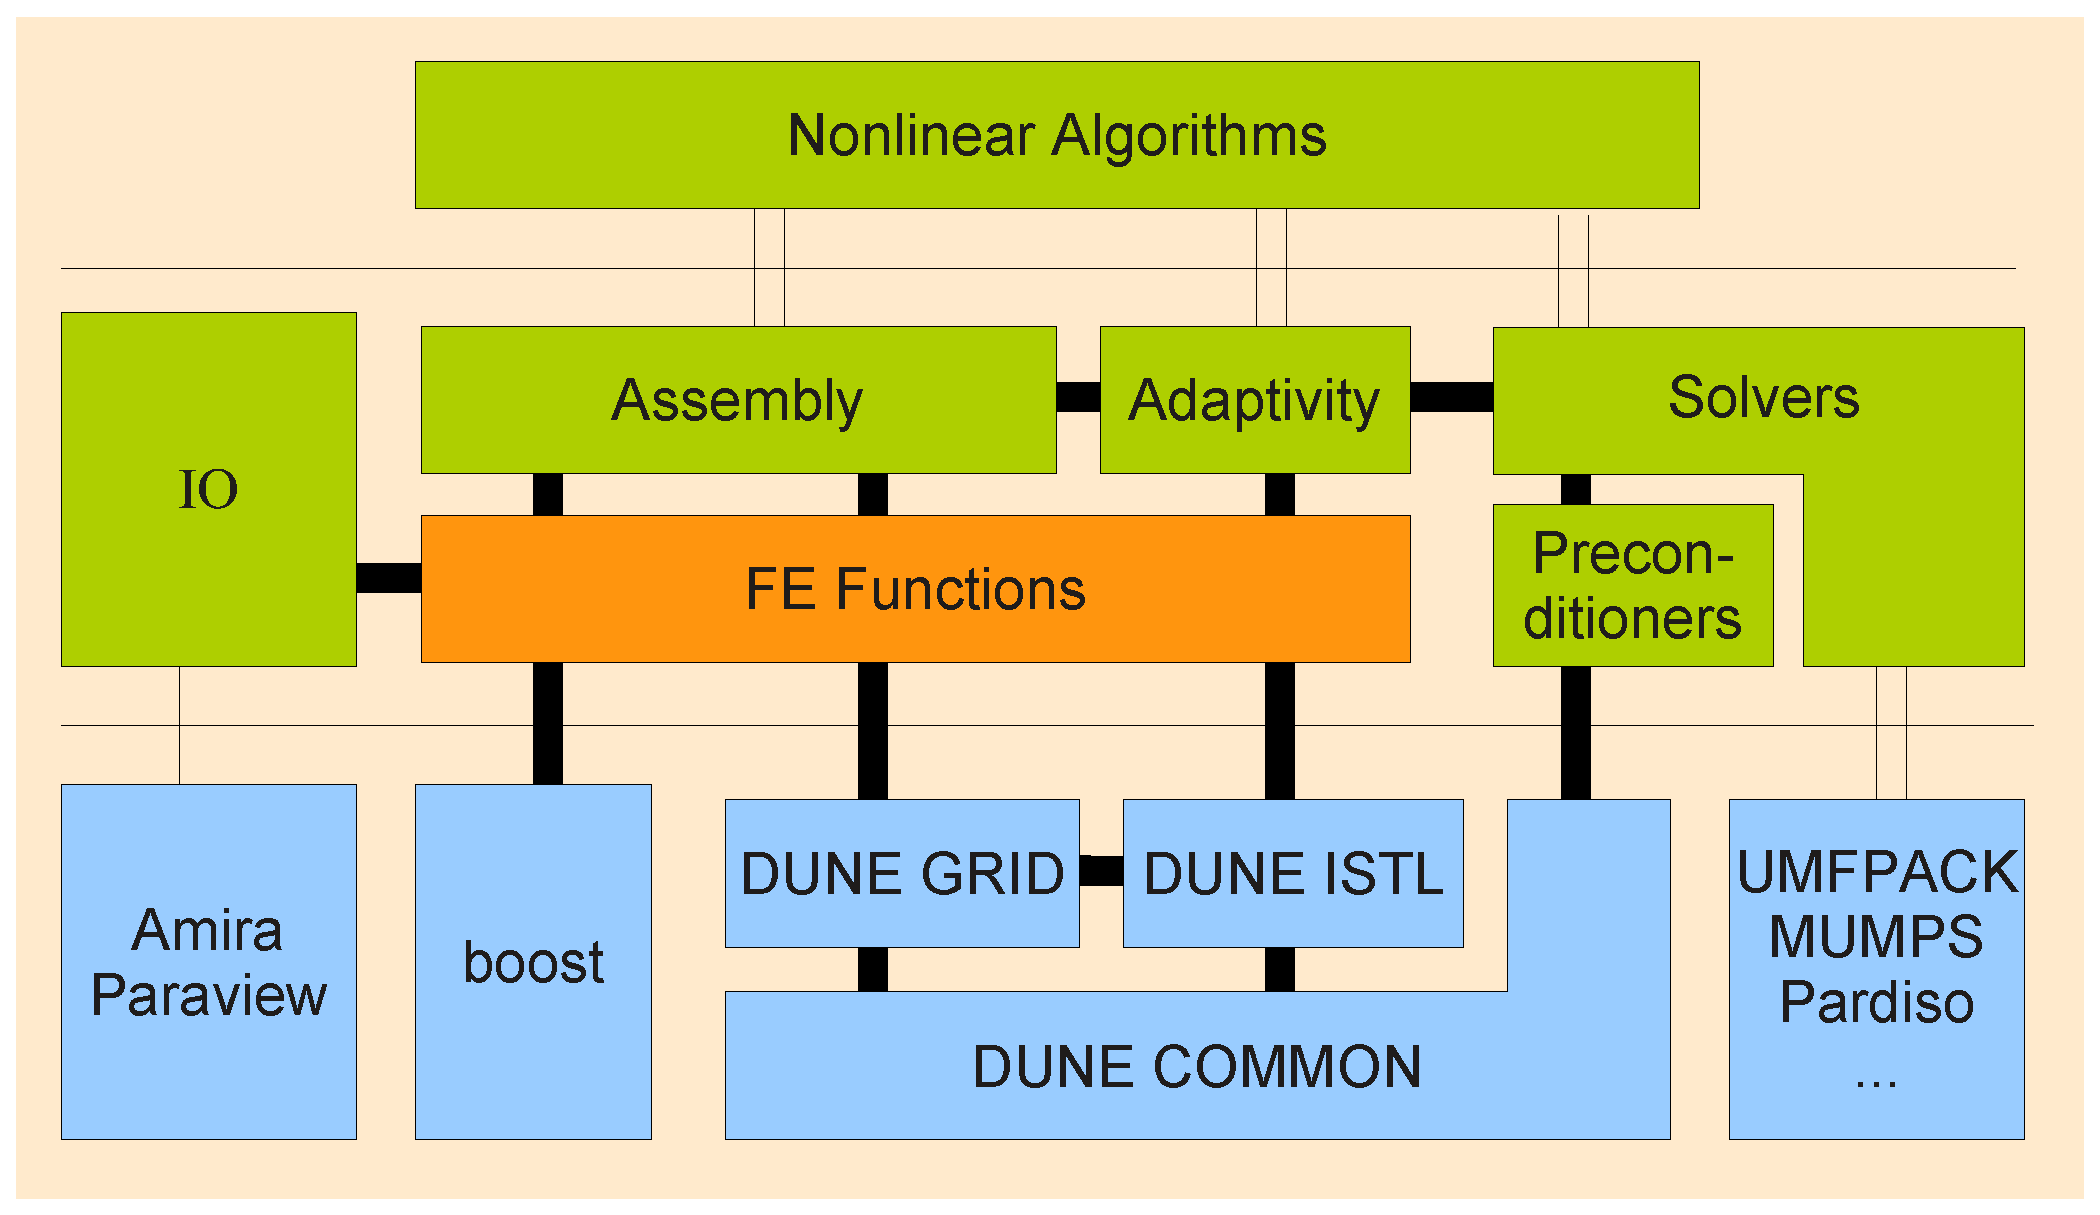
\includegraphics[scale=0.36]{kaskade7-2012-diagramm.eps}\\
  \vspace{-1mm}
   dynamic (\raisebox{0.7mm}{$\underline{\overline{\rule{0.6cm}{0pt}}}$}) and static  (\raisebox{0.2mm}{\rule{0.6cm}{0.1cm}}) polymorphism
  \caption{ Module interaction } \label{fig:modules}
\end{figure}


\section{Installation and code structure}\label{Install}

\subsection{Obtaining \K and third-party software}
\K is maintained by the Apache revision control system SVN and is hosted on the server {https://svn.zib.de/}.  
To obtain a working copy of \K from the ZIB SVN repository, change to the directory wherein you want to create 
the working copy subdirectory and enter the command 

\begin{scriptsize} 
\begin{verbatim} 
svn co https://user@svn.zib.de/zibDUNE/Kaskade7.3
\end{verbatim} 
\end{scriptsize} 

or

\begin{scriptsize} 
\begin{verbatim} 
svn co --username user https://svn.zib.de/zibDUNE/Kaskade7.3
\end{verbatim} 
\end{scriptsize} 


\noindent where you substitute {\tt user} 
by your ZIB SVN userid. If you intend to run 
your \K copy on a 64-bit Linux system at the ZIB (e.g., on a machine of the HTC cluster), just change into the \K directory, 
create a suitable file named {\tt Makefile.Local}, by creating a copy of {\tt Makefile-htc.Local} 
with this name and changing the macros {\tt KASKADE7} and for a non-htc machine also {\tt INSTALLS}. 
Set the environment variables {\tt PATH} and {\tt LD\_LIBRARY\_PATH} to suitable values (see below) 
and type 

\begin{scriptsize} 
\begin{verbatim} 
make install 
\end{verbatim} 
\end{scriptsize} 

\noindent If you intend to run \K on some other system, you need to install on this system a suitable 
compiler and other thirdparty software which is needed by \K. 
To fulfil this task, get from the ZIB repository the \K software installer by the following command 

\begin{scriptsize} 
\begin{verbatim} 
svn co https://user@svn.zib.de/zibDUNE/Install_Kaskade7
\end{verbatim} 
\end{scriptsize} 

\noindent Then change to the Install\_Kaskade7 directory and use some {\tt install-xxx.Local} file as a template for 
the {\tt install.Local} file which you need to create. Review the {\tt install.Local} file and perhaps adapt it to 
your installation needs (for example the name and location of your LAPACK/BLAS library). For a LINUX 64bit system, we
recommend to use the ACML library from http://developer.amd.com/tools-and-sdks/cpu-development/amd-core-math-library-acml/acml-downloads-resources/
as LAPACK/BLAS replacement. 
\newline Please, also read the file {\tt README\_BEFORE\_STARTING}, and check for availability of the prerequites mentioned in this file. Also, take special attention to other notes marked by $\ast\ast\ast$ . Doing so may perhaps save you a lot of time in case of unexpected errors during the installation run.
Finally, run the command 

\begin{scriptsize} 
\begin{verbatim} 
./install.sh
\end{verbatim} 
\end{scriptsize} 

\noindent The {\tt./install.sh} shellscript will prompt you for some needed information, and then install all required third-party software. As the last step, the shellscript will also create a suitable Makefile.Local in the \K directory, and run the commands 

\begin{scriptsize} 
\begin{verbatim} 
make install 
make tutorial 
\end{verbatim} 
\end{scriptsize} 

%If you have installed Alberta during the previous installation run, then before you can use Kaskade7.2 with AlbertaGrid, you will need to make some small
%modifications to header-files of Kaskade7.2 and some thirdpartysoftware. For details, read the file {\tt ALBERTA\_IMPORTANT\_HINTS.txt} in the installer-directory.

\subsection{Structure of the program}
After checking out the program to directory  KASKADE7 we have the following 
structure of the source code stored into corresponding subdirectories.

\begin{itemize}
\item KASKADE7/algorithm
\item KASKADE7/fem
\item KASKADE7/io
\item KASKADE7/ipopt                      %\hspace*{30mm}(headers only)
\item KASKADE7/linalg
\item KASKADE7/mg                         %\hspace*{30mm}(headers only)
\item KASKADE7/timestepping               %\hspace*{30mm}(headers only)
\item KASKADE7/tests
\item KASKADE7/tutorial
\item KASKADE7/problems
\item KASKADE7/experiments
\end{itemize}

\noindent In these subdirectories we find {\tt .hh-} and {\tt .cpp-} files, some auxiliary files and sometimes further subdirectories.
In directories including {\tt .cpp-} files there is a {\tt Makefile} generating object files or libraries which are stored into
{\tt KASKADE7/libs}.

\subsection{Compiler und Libraries}\label{sec:comp_and_lib}

Before calling {\tt make} in KASKADE7 directory or in one of the subdirectories
the user should make sure that the correct compiler (corresponding to the selection in the Makefiles)
is available. In the installation at ZIB this can be provided by modifying the
PATH variable, e.g.,

\begin{scriptsize}
\begin{verbatim}
setenv PATH /home/datanumerik/archiv/software/linux64/gcc-$VERSION_GCC/gcc/bin:$PATH
\end{verbatim}
\end{scriptsize}

\noindent where we have to set $\$VERSION\_GCC$ to "4.9.3" or "5.3.0" in version
7.3 of \K (note that the given paths (\verb|/home/datanumerik/|\dots) are adjusted to htc use).

\noindent In order to assure that all needed shared libraries are found we have to set the 
{\tt LD$\_$LIBRARY$\_$PATH} variable to the shared libraries 
libmpfr.so, libmpc.so, libgmp.so (used when the compiler is called):

\begin{scriptsize}
\begin{verbatim}
setenv LD_LIBRARY_PATH "//home/datanumerik/archiv/software/linux64/lib"
\end{verbatim}
\end{scriptsize}

\noindent or similar in a bash shell:

\begin{scriptsize}
\begin{verbatim}
LD_LIBRARY_PATH="/home/datanumerik/archiv/software/linux64/lib"
export LD_LIBRARY_PATH
\end{verbatim}
\end{scriptsize}

Note: on MacOS X machines we have to set the variable  {\tt DYLD$\_$LIBRARY$\_$PATH}
with the corresponding paths.

\subsection{Using the make command}
\paragraph{Makefile.Local.}
In the root directory {\tt KASKADE7} the user has to write a file {\tt Makefile.Local} including paths to third-party software, compilers,
as well as flags for compiler and debugger. In particular, the full path of the {\tt KASKADE7} directory has to be defined.
There are example files like {\tt Makefile-htc.Local} and {\tt Makefile-mac.Local} which can be copied and modified for use on HTC- resp. Mac-machines.


\paragraph{make in the KASKADE directory.}
In the root directory KASKADE the Makefile may be called with different parameters:
\begin{itemize}
\item {\bf make clean} removes all object files, executables, graphics out, and some other files.
\item {\bf make depend} generates the {\tt Makefile} in the \K subdirectories from the {\tt Makefile.gen} template, which includes dependencies to all (possibly nested) included c++ headerfiles of KASKADE.
\item {\bf make kasklib} generates object files and builds the library {\tt libkaskade.a}.
\item {\bf make install} combines the two commands {\it make depend} and {\it make kasklib}.
\item {\bf make tutorial} builds and executes the examples in the {\tt tutorial} , and builds the pdf version of the manual.
\item {\bf make cleantutorial} removes all object files, executables, and some other files in the {\tt subdirectories}.       
\item {\bf make test} builds and executes the examples in the {\tt benchmarking} subdirectories.
\item {\bf make distribution} generates tar.gz - files after executing {\bf make clean}, ignoring SVN information,
documentation, and particular subdirectories.
\end{itemize}

\noindent For installing the complete \K use the three top make commands from above in the order specified: 
{\bf clean}, {\bf depend}, {\bf kasklib}. 
Note, that first some shell variables (i.e., $PATH$ and $LD\_LIBRARY\_PATH$) 
have to be defined as described in the paragraph \ref{sec:comp_and_lib}.


\paragraph{make in subdirectory.}
Once you have a complete installation of \K it may be necessary (after changing a file) to recompile in
a subdirectory and update the \K library. This is done by using the file {\tt Makefile} in the
corresponding subdirectory. You just have to type {\tt make}.

Note, that after checking out the code from the repository there are no files {\tt Makefile} in 
the subdirectories but only files called {\tt Makefile.gen}. Such a {\tt Makefile.gen} can be used to
generate a corresponding {\tt Makefile} by typing:

\begin{itemize}
\item make -f Makefile.gen depend
\end{itemize}

\noindent Thus the \K header files dependencies are detected and registered in the {\tt Makefile}. 
Each {\tt Makefile.gen} includes
a {\tt depend} and a {\tt clean} option.
Note that a call {\bf make depend} in the KASKADE directory also generates the local {\tt Makefile} from
the local {\tt Makefile.gen} 
in each of the subdirectories mentioned in the {\tt Makefile}. 

\subsection{Examples}
Applications of the \K software can be found in the subdirectories

\begin{itemize}
\item KASKADE7/tutorial
\item KASKADE7/tests
\item KASKADE7/problems
\end{itemize}

\noindent Each of these subdirectories needs a {\tt Makefile.gen} with the properties mentioned above.
In the subdirectory {\tt KASKADE7/tutorial} you find examples which are described
in detail in this manual starting with Section \ref{examples}. 

%\noindent The subdirectory {\tt KASKADE7/experiments} includes more or less the same examples as
%the tutorial subdirectory. These examples uld be used to test any changes in the base code of \K{}. 
%No modification in the tutorial code should be committed to the svn repository
%\noindent The subdirectory {\tt KASKADE7/experiments/moreExamples} may be used for examples still under construction.

\noindent More examples can be
found in subdirectory KASKADE7/problems, but without annotation. In particular, you find
here the current projects of developers. 


\subsection{Testing}
The directory {\tt KASKADE7/tests} provides a set of test examples. 
In addition to the examples in the tutorial we investigate here not only whether the 
computation is running but also whether it computes the correct results.

\noindent The testing is started in the \K root directory by typing
\begin{itemize}
\item {\bf make test}
\end{itemize}

\noindent The results will be summarized in the file {\tt testResult.txt}.

\subsection{Communication with svn repository}\label{svn}
Above in this section we described how to get a copy from the \K repository by 
the shell command

\begin{scriptsize} 
\begin{verbatim} 
svn co https://user@svn.zib.de/zibDUNE/Kaskade7.3
\end{verbatim} 
\end{scriptsize} 

\noindent This copy can be used for arbitrary applications. Any change by the user is allowed.
But it is always under certain control of the svn system, i.e. the version control system svn registers
all differences between repository and local copy.
Furthermore, svn provides a set of commands to 
communicate between the local copy of a user and the current state
of the repository. Thus there are svn commands to add a new file
into the repository, to delete a file from the repository, to update
local files or to commit local changes to the repository.

Enter the command 

\begin{scriptsize} 
\begin{verbatim} 
svn help
\end{verbatim} 
\end{scriptsize} 

\noindent in your shell to get a first idea of the options offered by svn:

\begin{scriptsize} 
\begin{verbatim} 
%svn help
usage: svn <subcommand> [options] [args]
Subversion command-line client, version 1.6.17.
Type 'svn help <subcommand>' for help on a specific subcommand.
Type 'svn --version' to see the program version and RA modules
 or 'svn --version --quiet' to see just the version number.

Most subcommands take file and/or directory arguments, recursing
on the directories.  If no arguments are supplied to such a
command, it recurses on the current directory (inclusive) by default.

Available subcommands:
  add
  blame (praise, annotate, ann)
  cat
  changelist (cl)
  checkout (co)
  cleanup
  commit (ci)
  copy (cp)
  delete (del, remove, rm)
  diff (di)
  export
  help (?, h)
  import
  info
  list (ls)
  lock
  log
  merge
  mergeinfo
  mkdir
  move (mv, rename, ren)
  propdel (pdel, pd)
  propedit (pedit, pe)
  propget (pget, pg)
  proplist (plist, pl)
  propset (pset, ps)
  resolve
  resolved
  revert
  status (stat, st)
  switch (sw)
  unlock
  update (up)

Subversion is a tool for version control.
For additional information, see http://subversion.tigris.org/
%
\end{verbatim} 
\end{scriptsize} 

\noindent The correct syntax of all these svn commands can easily be found
in the internet, e.g., {\tt http://subversion.tigris.org/}.


\section{External libraries}\label{libs}

\begin{itemize}
\item ALBERTA: Directory alberta-3.0.1/lib (optional)
\begin{itemize}
\item  {\bf libalberta\_3d.a} \newline
    ALBERTA 3D-grid routines.
\item  {\bf libalberta\_2d.a} \newline
    ALBERTA 2D-grid routines.
\item  {\bf libalberta\_1d.a} \newline
    ALBERTA 1D-grid routines.
\item  {\bf libalberta\_utilities.a} \newline
    ALBERTA common utilities routines.
\end{itemize}
\item AMIRAMESH: Directory libamira/lib (license restrictions apply!)
\begin{itemize}
\item  {\bf libamiramesh.a}  \newline
       Reading and writing Amiramesh files.
\end{itemize}
\item BOOST: Directory boost-1.59.0/lib
\begin{itemize}
\item  {\bf libboost\_signals.SUFFIX} \newline
       Managed signals and slots callback implementation.
\item  {\bf libboost\_program\_options.SUFFIX} \newline
       The program\_options library allows program developers to obtain program options, that is (name, value) pairs from the user, via conventional methods such as command line and config file.
\item  {\bf libboost\_program\_system.SUFFIX} \newline
       Operating system support, including the diagnostics support that will be part of the C++0x standard library.
\item  {\bf libboost\_program\_timer.SUFFIX} \newline
       Event timer, progress timer, and progress display classes.
\item  {\bf libboost\_program\_thread.SUFFIX} \newline
       Portable C++ multi-threading.
\item  {\bf libboost\_program\_chrono.SUFFIX} \newline
       Useful time utilities.
       
\item {\bf SUFFIX} is {\bf so} under Linux and {\bf dylib} under MacOS X (Darwin)
\end{itemize}
\item DUNE: Directory dune-2.4.1/lib
\begin{itemize}
\item  {\bf libdunecommon.a} \newline
       DUNE common modules.
\item  {\bf libdunegeometry.a} \newline
       DUNE geometry modules.
\item  {\bf libdunegrid.a} \newline
       DUNE grid methods.
\item  {\bf libdunealbertagrid\_3d.a} \newline
       DUNE interface to ALBERTA 3D-grid routines. (optional)
\item  {\bf libdunealbertagrid\_2d.a} \newline
       DUNE interface to ALBERTA 2D-grid routines. (optional)
\item  {\bf libdunealbertagrid\_1d.a} \newline
       DUNE interface to ALBERTA 1D-grid routines. (optional) 
\item  {\bf libdunegridglue.a} \newline
       DUNE library for contact-problems (optional)
\end{itemize}
\item HYPRE: Directory hypre-2.6.0b/lib
\begin{itemize}
\item  {\bf libHYPRE.a}
\end{itemize}
\item ITSOL: Directory itsol-1/lib
\begin{itemize}
\item  {\bf libitsol.a}
\end{itemize}
\item MUMPS: Directory mumps-4.10.0/lib \newline
      Direct sparse linear solver library.
\begin{itemize}
\item  {\bf libdmumps.a}
\item  {\bf libmpiseq.a}
\item  {\bf libmumps\_common.a}
\item  {\bf libpord.a}
\item  {\bf libpthread.a}
\end{itemize}
\item SUPERLU: Directory superlu-4.3/lib \newline
      Direct sparse linear solver library.\newline
      (Dropped from list of supported libraries due to danger of potential mixup with (a bit older) SuperLU routines which are included in the HYPRE library)
\begin{itemize}
\item  {\bf libsuperlu.a}
\end{itemize}
\item TAUCS: Directory taucs-2.0/lib \newline
      Preconditioner library.
\begin{itemize}
\item  {\bf libtaucs.a}
\end{itemize}
\item UG for DUNE: Directory dune-2.4.1/lib \newline
       UG for DUNE, FEM grid-library.
\begin{itemize}
\item  {\bf libugS3.a}
\item  {\bf libugS2.a}
\item  {\bf libugL3.a}
\item  {\bf libugL2.a}
\item  {\bf libdevS.a}
\item  {\bf libdevX.a}
\end{itemize}
\item UMFPACK: Directory umfpack-5.4.0/lib \newline
      Direct sparse linear solver library.
\begin{itemize}
\item  {\bf libumfpack.a}
\item  {\bf libamd.a}
\end{itemize}
\end{itemize} 

\section{Documentation online}\label{docu}
In subdirectory {\em Kaskade7/doc} there is a script {\em makeDocu} for generating a documentation 
of the source code. Necessary is the program {\em doxygen} and a {\em Latex} installation.
Outline and shape of the documentation is steered by the {\em doxygen} parameter file  called {\em Doxyfile}.

By default ( $GENERATE\_HTML = YES$ ) the generation of HTML pages is selected. The source files to be analysed are
defined via {\em INPUT} variable.

If the auxiliary program {\em dot} of the {\em GraphViz} software is available, we recommend to change the 
preset $HAVE\_DOT = NO$ to $HAVE\_DOT = YES$ in the file {\em Doxyfile}.


After generating the documentation ( by command {\em makeDocu} ) the pages may be considered
in the browser by specifying the full path $.../kaskade7/doc/html/index.html$.


\section{Getting started}\label{examples}
In this chapter we present a set of examples which enables a user wihout any experience
with \K to get started. In particular, the first example specifies all the steps needed to
understand the technical handling of \K independent of any know-how about numerics and implementation.
The following examples give more and more details, bringing together the mathematical
formulation of a problem and its implementation.



\subsection{A very first example: simplest stationary heat transfer}\label{Laplace}
This example is implemented in subdirectory 
\begin{center} KASKADE7/tutorial/laplacian\end{center}

\noindent Files: {\bf laplace.cpp}, {\bf laplace.hh}, {\bf Makefile}

\noindent We compute the solution $u$ of the Laplacian or Poisson equation

\begin{equation}\label{PDE_Laplace}
\begin{array}{rcl}
 -\nabla  \cdot (\nabla u) = 1 \quad &\mbox{x }\in  \Omega\\[2mm]
u = 0 \quad & \mbox{on } \Gamma
\end{array}
\end{equation}

\noindent on the two-dimensional open unit square $\Omega$ under homogeneous boundary conditions
on $\Gamma = \partial \Omega$. These equations may describe  stationary heat transfer caused by a
constant heat source (value 1 on the right-hand side) 
and constant temperature ($0 ^{o} C$) on the boundary, e.g. by cooling.

Resolving the $\nabla$ - operator in the equation (\ref{PDE_Laplace}), we can also write it in Cartesian coordinates $x$ and $y$

\begin{equation}\label{PDE_LaplaceXY}
\begin{array}{rcl} \displaystyle
 - \frac{\partial^2 u}{ \partial x^2} - \frac{\partial^2 u}{ \partial y^2} = 1 \quad &(x,y)  \in  (0,\,1)^2\\[2mm]
u = 0 \quad & \mbox{on } \Gamma
\end{array}
\end{equation}


The treatment of this problem in context of finite element methods as used in \K is based
on a variational formulation of the equation (\ref{PDE_Laplace}) and needs to provide 
a triangulation of the domain $\bar\Omega$ (including the boundary),
a set of ansatz functions (order 1: linear elements, order 2: quadratic elements,...), functions for
evaluating the integrands in the weak formulation, assembling of the stiffness matrix and right-hand side.
All this is to be specified in the files {\em laplace.cpp} and {\em laplace.hh} using the functionality
of the \K library. Shortly, we will explain the details and possibilities to change the code.

Once appropriate changes are made to the code, the user has to compile and generate the executable by calling the {\em Makefile} (recall that the {\em Makefile} was already generated during the installation process as introduced in Section \ref{Install}) and is in the same directory. Just enter the command

\begin{scriptsize}
\begin{verbatim}
make laplace
\end{verbatim}
\end{scriptsize}

\noindent or simply

\begin{scriptsize}
\begin{verbatim}
make
\end{verbatim}
\end{scriptsize}

\noindent If this {\em make} procedure works without errors you get the executable file {\em laplace} 
which can be run by the command

\begin{scriptsize}
\begin{verbatim}
./laplace
\end{verbatim}
\end{scriptsize}

\noindent The program sends some messages to the terminal (about progress of the calculation)
and writes graphical information (mesh and solution data) 
to a file {\em temperature.vtu}. This file can be visualized by any tool (e.g., {\em paraview})
which can interprete vtk format.

The shell command

\begin{scriptsize}
\begin{verbatim}
make clean
\end{verbatim}
\end{scriptsize}

\noindent deletes the files {\em laplace}, {\em laplace.o}, {\em temperature.vtu}, and {\em gccerr.txt}.
The last one is only generated if errors or warnings are discovered by the compiler. Then it includes all the
error messages and warnings in a single file which offers a more comfortable way to analyse the errors than to get all error messages at once on the terminal.

We summarize:
In order to get a running code which computes a finite element soluton of the Lapacian problem
(\ref{PDE_Laplace}) the following three commands

\begin{scriptsize}
\begin{verbatim}
make clean
make 
./laplace
\end{verbatim}
\end{scriptsize}

\noindent have to be entered.

Now we explain the fundamentals of treating problems like (\ref{PDE_Laplace}) in \textsc{Kaskade7}.
Using the notation from Section \ref{problemDef} we define for this example
\[
F(u) := \frac{1}{2}\nabla u^T \nabla u  -  f u
\]
and 
\[
G(u) := \gamma\frac{1}{2} (u-u_0)^2, \quad u_0 = 0
\]
with a (large, e.g., $10^9$) penalty factor $\gamma$ ensuring sufficiently accurate satisfaction of the Dirichlet boundary condition.
%Solving Equation (\ref{PDE_Laplace}) results in:



%The main step is that the problem may also be given in the {\em weak} formulation:
%
%Find a solution $u$ of
%
%\begin{equation}\label{weakForm}
%  \int_{\Omega} \nabla u^T \nabla v  \, dx = \int_{\Omega} f v \,dx   \quad\quad \forall v \in H_0^1(\Omega)
%\end{equation}
%
%\noindent with $f = 1$ in our example. Here we neglect the boundary conditions.
%
%Using the notation of the general  problem formulation in Subsection \ref{problemDef}
%
%\begin{equation}\label{weakForm2}
%  a(u,v) = \langle f,v\rangle  \quad\quad \forall v \in H_0^1(\Omega)
%\end{equation}
%
%\noindent with the bilinear form $a(u,v) = \int_{\Omega} \nabla u^T \nabla v  \, dx$ and the
%functional $\langle f,v\rangle  = \int_{\Omega} f v \,dx$. 
%
%
%In addition, a solution $u$ of equation (\ref{weakForm2}) is also a minimizer of the functional
%
%\[
%\Phi(v) = \frac{1}{2} a(v,v) - \langle f,v\rangle =  \int_{\Omega} (\frac{1}{2}\nabla v^T \nabla v  -  f v) \,dx
%\]
%
%i.e.,
%
%\[
%  \Phi(u) = \min_{v \in H_0^1(\Omega)} \left\{\frac{1}{2} a(v,v) - \langle f,v\rangle\right\}  
%\]
%
%Also considering the boundary condition $g(x,v)$ on $\partial \Omega$ we have to complete
%\begin{equation}\label{minFunc}
%  \Phi(u) = \min_{v \in H_0^1(\Omega)} \left\{\frac{1}{2} a(v,v) - \langle f,v\rangle + \int_{\partial\Omega} g(v)   \, ds\right\}
%\end{equation}

\noindent We compute a solution of the minimization problem (\ref{basicvariational}) by a Newton iteration solving in each step the following problem:

Find $u \in V \subset H_0^1(\Omega)$ such that 

\[
  \int_{\Omega} d2^{\Omega}(u,v) \, dx + \int_{\Gamma} d2^{\Gamma}(u,v) \, ds = 
  -\int_{\Omega} d1^{\Omega}(v) \,dx  - \int_{\Gamma} d1^{\Gamma}(v) \,ds \quad\quad \forall v \in V,
\]

\noindent with $d1^{\Omega}(v) = F'(\cdot)v$, $d2^{\Omega}(u,v) = F''(\cdot)[u,v]$, $d1^{\Gamma}(v) = G'(\cdot)v$, and $d2^{\Gamma}(u,v) = G''(\cdot)[u,v]$
where $u$ is the Newton update (being $\delta u$ in section \ref{problemDef}).

In our context $V$ is always a finite element space spanned by the base functions $\{\varphi_i\}_{1,\dots,N}$,with $N$ as the dimension of the space.
That means, we have to solve the following system of $N$ equations in order to find the minimum in the space $V$:

\begin{equation}\label{weakFunc}
  \int_{\Omega} d2^{\Omega}(u,\varphi_i) \, dx + \int_{\Gamma} d2^{\Gamma}(u,\varphi_i) \, ds = 
  \int_{\Omega} d1^{\Omega}(\varphi_i) + \int_{\Gamma} d1^{\Gamma}(\varphi_i)\,ds   \quad\quad \mbox{for}\quad \varphi_i,\ i=1,\dots,N.
\end{equation}

\noindent Here we have 
\begin{eqnarray}{}
d0^{\Omega}() &=& \frac{1}{2} \nabla u^T \nabla u  -  f u\\
d1^{\Omega}(\varphi_i) &=& \nabla u^T \nabla \varphi_i - f \varphi_i \\
d2^{\Omega}(\varphi_i,\varphi_j) &=& \nabla \varphi_i^T \nabla \varphi_j
\end{eqnarray}

\noindent in the region $\Omega$, and 

\begin{eqnarray}{}
d0^{\Gamma}() &=& \gamma \ \frac{1}{2} (u - u_0)^2\\
d1^{\Gamma}(\varphi_i) &=& \gamma \ (u - u_0) \varphi_i \\
d2^{\Gamma}(\varphi_i,\varphi_j) &=& \gamma \ \varphi_i  \varphi_j
\end{eqnarray}

\noindent on the boundary $\Gamma$.

These functions have to be defined in two mandatory classes in the problem class
(called HeatFunctional):
the {\em DomainCache} defining $d0^{\Omega}()$, $d1^{\Omega}()$, and $d2^{\Omega}()$ for the region $\Omega$, and the 
{\em BoundaryCache} defining $d0^{\Gamma}()$, $d1^{\Gamma}()$, and $d2^{\Gamma}()$ on the boundary $\Gamma = \partial \Omega$.

In general the functional to be minimized depends nonlinearly on the solution $u$.
However, in this example it is linear, hence the first step of  Newton's method already
provides the solution and is implemented in {\em main()} as shown below. In case of a nonlinear
functional we have to write a complete Newton loop controlling the size of the update and stopping
if it is small enough. We present such an example (from elasticity) later in this chapter.


Now, we focus on the specific details of implementation for our Laplacian problem which can be
found in the files {\em laplace.cpp} and {\em laplace.hh}.
We are not trying to explain everything. Just some hints to the essentials in order to get a first
feeling for the code.

The code in the main program (file {\em laplace.cpp})

%\begin{scriptsize}
%\begin{verbatim}
\begin{lstlisting}
int main()
{
  std::cout << "Start Laplacian tutorial program" << std::endl;

  constexpr int dim = 2;
  int refinements = 5,
      order       = 2;

  using Grid = Dune::UGGrid<dim>;
  using LeafView = Grid::LeafGridView;
  using H1Space = FEFunctionSpace<ContinuousLagrangeMapper<double,LeafView> >;
  using Spaces = boost::fusion::vector<H1Space const*>;
  using VariableDescriptions = boost::fusion::vector<Variable<SpaceIndex<0>,Components<1>,VariableId<0> > >;
  using VariableSetDesc = VariableSetDescription<Spaces,VariableDescriptions>;
  using Functional = HeatFunctional<double,VariableSetDesc>;
  using Assembler = VariationalFunctionalAssembler<LinearizationAt<Functional> >;
  using Operator = AssembledGalerkinOperator<Assembler>;
  using CoefficientVectors = VariableSetDesc::CoefficientVectorRepresentation<0,1>::type;

  ...
}
\end{lstlisting}
%\end{verbatim}
%\end{scriptsize}

\noindent sets some parameters and \emph{using} statements and comprises the following essential parts:
\begin{itemize}
\item definition of a triangulation of the region $\Omega$
%\begin{scriptsize}
%\begin{verbatim}
\begin{lstlisting}
  GridManager<Grid> gridManager( createUnitSquare<Grid>() );
  gridManager.globalRefine(refinements);
\end{lstlisting}
%\end{verbatim}
%\end{scriptsize}

The parameter {\em refinements} defined in top of the main program
determines how often the coarse grid defined here has to be refined uniformly.
The resulting mesh is the initial one for the following computation.
In context of adaptive mesh refinement it might be object of further refinements,
see example in subsection \ref{EmbeddEsti}.


\item definition of the finite element space
%\begin{scriptsize}
%\begin{verbatim}
\begin{lstlisting}
  // construction of finite element space for the scalar solution u.
  H1Space temperatureSpace(gridManager,gridManager.grid().leafView(),order);
  Spaces spaces(&temperatureSpace);
  VariableSetDesc variableSetDesc(spaces,{ "u" });
\end{lstlisting}
%\end{verbatim}
%\end{scriptsize}

Here we define the finite element space underlying the discretization of our
equation (\ref{weakFunc}) corresponding to the introduction in Section \ref{FEspaces}.
The parameter {\em order} defined in top of the main program specifies the
order of the finite element space in the statement 

%\begin{scriptsize}
%\begin{verbatim}
\begin{lstlisting}
H1Space temperatureSpace(gridManager,gridManager.grid().leafView(),order);
\end{lstlisting}
%\end{verbatim}
%\end{scriptsize}



\item definition of the variational functional
%\begin{scriptsize}
%\begin{verbatim}
\begin{lstlisting}
Functional F;
\end{lstlisting}
%\end{verbatim}
%\end{scriptsize}

The code defining the functional  can be found in the file {\em laplace.hh}.
The corresponding class is called {\em HeatFunctional} and contains the 
mandatory members {\em DomainCache} and {\em BoundaryCache} each of them specifying
the functions $d0()$, $d1()$, and $d2()$ described above. 
The static member template class $D2$ defines which Hessian blocks are available
what is of major interest in case of systems of equations, here we only have one block.
$D1$ provides information about the structure of the right-hand side, e.g., if
it is non-zero (present = true, i.e. it is present) or if it is not constant (constant = false).
In the member function {\em integrationOrder} the order of the integration formula used
in the assembling is specified.

%\begin{scriptsize}
%\begin{verbatim}
\begin{lstlisting}
template <class RType, class VarSet>
class HeatFunctional : public FunctionalBase<VariationalFunctional>
{
public:
  using Scalar = RType;
  using OriginVars = VarSet;
  using AnsatzVars = VarSet;
  using TestVars = VarSet;

  class DomainCache : public CacheBase<HeatFunctional,DomainCache>
  {
   ...
  }

  class BoundaryCache : public CacheBase<HeatFunctional,BoundaryCache>
  {
   ...
  }

  template <int row>
  struct D1 : public FunctionalBase<VariationalFunctional>::D1<row>
  {
    static bool const present   = true;
    static bool const constant  = false;
  };
  

  template <int row, int col>
  struct D2 : public FunctionalBase<VariationalFunctional>::D2<row,col>
  {
    static bool const present = true;
    static bool const symmetric = true;
    static bool const lumped = false;
  };


  template <class Cell>
  int integrationOrder(Cell const& /* cell */,
                       int shapeFunctionOrder, bool boundary) const 
  {
    if (boundary) 
      return 2*shapeFunctionOrder;
    else
    {
      int stiffnessMatrixIntegrationOrder = 2*(shapeFunctionOrder-1);
      int sourceTermIntegrationOrder = shapeFunctionOrder;  // as rhs f is constant, i.e. of 
                                                                                     order 0

      return std::max(stiffnessMatrixIntegrationOrder,sourceTermIntegrationOrder);
    }
  }
};
\end{lstlisting}
%\end{verbatim}
%\end{scriptsize}

The DomaineCache provides member functions $d0$, $d1\_impl$, and $d2\_impl$ evaluating  $F(\cdot )$, $F'(\cdot ) \varphi_i$,
$F''(\cdot ) [ \varphi_i,\varphi_j ]$, respectively.
The function $u$ is specified on construction of the caches, and can be evaluated for each quadrature point 
in the member function {\em evaluatedAt()} using the appropriate one among the evaluators provided by the assembler

%\begin{scriptsize}
%\begin{verbatim}
\begin{lstlisting}
  class DomainCache : public CacheBase<HeatFunctional,DomainCache>
    {
    public:
      DomainCache(HeatFunctional const&,
                  typename AnsatzVars::Representation const& vars_,
                  int flags=7):
        data(vars_)
      {}
  
  
      template <class Position, class Evaluators>
      void evaluateAt(Position const& x, Evaluators const& evaluators)
      {
        u  = component<uIdx>(data).value(boost::fusion::at_c<uSpaceIdx>(evaluators));
        du = component<uIdx>(data).derivative(boost::fusion::at_c<uSpaceIdx>(evaluators));
        f = 1.0;
      }
  
      Scalar
      d0() const
      {
        return sp(du,du)/2 - f*u;
      }
  
      template<int row>
      Scalar d1_impl (VariationalArg<Scalar,dim,TestVars::template Components<row>::m> const& arg) const
      {
        return sp(du,arg.derivative) - f*arg.value;
      }
  
      template<int row, int col>
      Scalar d2_impl (VariationalArg<Scalar,dim,TestVars::template Components<row>::m> const &argTest,
                      VariationalArg<Scalar,dim,AnsatzVars::template Components<row>::m> const &argAnsatz) const
      {
        return sp(argTest.derivative,argAnsatz.derivative);
      }
  
    private:
      typename AnsatzVars::Representation const& data;
      Dune::FieldVector<Scalar,AnsatzVars::template Components<uIdx>::m> u, f;
      Dune::FieldMatrix<Scalar,AnsatzVars::template Components<uIdx>::m,dim> du;
      LinAlg::EuclideanScalarProduct sp;
    };
\end{lstlisting}
%\end{verbatim}
%\end{scriptsize}


The {\em BoundaryCache} is defined analogously.
More details are presented in the next examples.
We now continue with the \emph{laplace.cpp} file.


\item assembling and solution of a linear system
%\begin{scriptsize}
%\begin{verbatim}
\begin{lstlisting}
  //construct Galerkin representation
  Assembler assembler(spaces);
  VariableSetDesc::Representation u(variableSetDesc);
  assembler.assemble(linearization(F,u));

  Operator A(assembler);
  CoefficientVectors solution(VariableSetDesc::CoefficientVectorRepresentation<>::init(spaces));
  CoefficientVectors rhs(assembler.rhs());

  directInverseOperator(A).applyscaleadd(-1.0,rhs,solution);
  component<0>(u) = component<0>(solution);
\end{lstlisting}
%\end{verbatim}
%\end{scriptsize}

The {\em assembler} is the kernel of each finite element program. It evaluates
the integrals of the weak formulation based on the member functions of the HeatFunctional
class and the finite element element space defined in the {\em H1Space} from above, of course
closely aligned to the {\em Grid}.

\item output for graphical device and end of program
%\begin{scriptsize}
%\begin{verbatim}
\begin{lstlisting}
  writeVTKFile(u,"temperature",IoOptions().setOrder(order).setPrecision(7));

  std::cout << "graphical output finished, data in VTK format is written into file temperature.vtu \n";
  std::cout << "End Laplacian tutorial program" << std::endl;
\end{lstlisting}
% \end{verbatim}
% \end{scriptsize}

\K offers two formats to specify output of mesh and solution data for graphical devices.
The VTK format is used in this example and can be visualized  by {\em Paraview} software, for example.
In particular for 3D geometries the format of the visualization package {\em amira} is
recommended.

\end{itemize}


\noindent {\bf Exercises}:

1. Use the parameter {\em refinements} to generate grids of different refinement levels. Write the
grid and solution data into a file and compare the results by a visualization tool, e.g., {\em Paraview}.

2. In the example above we use quadratic finite elements of Lagrange type (i.e., {\em order} = 2).
Consider increase of the number of degrees of freedom for  {\em order} = 1,2,3,...

3. Change the value of \emph{f} in the header file (i.e. in the \emph{evaluateAt} member function) and
observe the changes in the output. (If there is no visible change, also look at the color legend.)

\vspace{1em}
\noindent {\bf Remark}: This first example has been updated in March 2015 (to which this tutorial is adjusted).
The following examples have not been updated so far which leads to discontinuities in coding/notation (e.g.
\emph{typedef} instead of \emph{using}).
In general the coding style of this example is to be followed.

\subsection{Example: stationary heat transfer}\label{StatHeat}

This example is implemented in subdirectory 
\begin{center} KASKADE7/tutorial/stationary\_heattransfer\end{center}

\noindent Files: {\bf ht.cpp}, {\bf ht.hh}, {\bf Makefile}

\noindent We consider another stationary heat transfer problem but with some
extensions compared to the preceding example:

\begin{itemize}
\item the region $\Omega$ may be two- or three-dimensional,
\item the diffusion coefficient $\kappa$ may depend on $x \in \Omega$,
\item the operator may include a mass term with coefficient $q(x), x \in \Omega$,
\item the heat source (right-hand side of heat transfer equation) may depend on $x \in \Omega$,
\item the user may select between direct and iterative solution of the linear systems,
\item the user gets support to handle parameters.
\end{itemize}

\noindent The corresponding scalar partial differential equation is still linear and given by


\begin{equation}\label{PDE_statHT}
\begin{array}{rcl}
 -\nabla  \cdot (\kappa(x) \nabla u) + q(x) u = f(x) \quad &\mbox{x }\in  \Omega\\[2mm]
\kappa  \displaystyle \frac{\partial u}{\partial n} = 0 \quad & \mbox{on } \Gamma_1\\[3mm]
u = u_b(x) \quad & \mbox{on } \Gamma_2
\end{array}
\end{equation}

\noindent $\Gamma_1$ and $\Gamma_2$ denote parts of the boundary $\partial \Omega = \Gamma_1\dot{\cup} \Gamma_2$ where we have to define 
boundary conditions. On $\Gamma_1$ we assume a homogeneous Neumann and on 
$\Gamma_2$ we prescribe the values of the solution $u$ (Dirichlet condition).

In \K, the solution of this problem is  FinitElement Method (FEM). Therefore it is necessary to consider
the system (\ref{PDE_statHT}) in its weak formulation, see appendix. In particular, we want to treat the problem in its
minimization formulation as in the example before and as described in Section \ref{problemDef} for the general case:

Find the solution $u$ of the minimization problem (in the finite element space) as described in (\ref{basicvariational}) using

\[
F(v) = \frac{1}{2} (\kappa \nabla v^T \nabla v + q v v)  -  f v
\]

\noindent and 
\[
G(v) = \frac{1}{2} (v-u_0)^2, \quad u_0 = u_b(x)
\]

\noindent We remark that the homogeneous Neumann boundary conditions provide no contribution in the weak formulation.

%\begin{equation}
%\label{PDE_Functional}
%J(u) = \min_{v} \{B(v,v)/2-F(v)\}
%\end{equation}
%
%\noindent using 
%
%\begin{equation}\label{PDE_minimization}
%\begin{array}{rcl}
%B(v,v)& = & \displaystyle  \int_{\Omega}\kappa \nabla v \nabla v dx  - \int_{\Omega}q(x)v vdx \vspace*{2mm}\\
%F(v) & = & \int_{\Omega}fvdx.
%\end{array}
%\end{equation}

\subsubsection{A walk through the main program}

For solving the problem we have to do both defining the attributes of the equations (\ref{PDE_statHT}) and defining the details of the method.
%The complete references are the sources {\tt ht.cpp} and {\tt ht.hh} in the directory {\tt tutorial/stationary\_heattransfer/}.
In order to keep the example simple we choose a constant diffusion coefficient $\kappa=1$, a constant mass coefficient $q=1$.
The right-hand side $f$ is determined so that $u = x(x-1)exp(-(x-0.5)^2)$ is solution of equation (\ref{PDE_statHT}) for all
$(x,y,z) \in \Omega$. The domain $\Omega$ is the square unit or unit cube respectively. On the boundary we have 
$u_b =0$ for $x=0$ and $x=1$, elsewhere homogeneous Neumann boundary conditions.

\paragraph{Preliminaries.}
We write some important parameters in the top of the main program, e.g., {\em order} defining the order of the finite element ansatz, 
or {\em refinements} specifying the number of refinements of the initial grid, or {\tt verbosity} for selecting the level 
(possible values 0,1,2,3) of
verbosity of certain functions (e.g. iterative solver).

%\begin{scriptsize}
%\begin{verbatim}
\begin{lstlisting}
int verbosityOpt = 1;
bool dump = true; 
std::unique_ptr<boost::property_tree::ptree> pt = 
getKaskadeOptions(argc, argv, verbosityOpt, dump);

int refinements = getParameter(pt, "refinements", 5),
    order 	= getParameter(pt, "order", 2),
    verbosity 	= getParameter(pt, "verbosity", 1);
std::cout << "original mesh shall be refined : " << refinements << " times" << std::endl;
std::cout << "discretization order : " << order << std::endl;
std::cout << "output level (verbosity): " << verbosity << std::endl;

int  direct, onlyLowerTriangle = false;

DirectType directType;
MatrixProperties property = SYMMETRIC;
PrecondType precondType = NONE;
std::string empty;
\end{lstlisting}
%\end{verbatim}
%\end{scriptsize}

\noindent In this example we use the function  $getKaskadeOptions$ to create 
a $property\_tree$ $pt$ for storing a set of parameters in tree structure. This tree is filled by predefinitions in 
a  file {\em default.json} and
 by  arguments in $argc$, $argv$. Based on this $property\_tree$
the call of $getParameter(..,s,..)$  
provides a value corresponding to the string $s$.
The result might be another string or a value of any other type, e.g. {\em integer} or {\em double}.
In particular, a parameter may be specified in the input line via the $argc$, $argv$ 
when starting the executable, e.g.,
\begin{itemize}
\item Let's have the following call of the executable {\tt heat}

{\tt  ./heat --order 1 }

then call of getParameter(...) in the statement

{\tt  order =  getParameter(pt, "order", 2);}

assign the value $1$ to the variable {\em order}. 

\item Let's start the executable without parameter list
then the call of getParameter(...) in the statement

{\tt  order =  getParameter(pt, "order", 2);}

checks for a string {\tt order} in the file {\tt Kaskade7/default.json}.
If there is none the default value of the getParameter(...,2) is assigned
to the variable {\em order}.

\item Let's  consider the following call of the executable

{\tt  ./heat --solver.type direct }

then call of getParameter(...) in the statement

{\tt getParameter(pt, "solver.type", empty);}

reveals the string "direct" as return value which is used to build a
 string $s$ by
 
{\tt std::string s("names.type.");}\\
{\tt s += getParameter(pt, "solver.type", empty);}

As result we get  "names.type.direct" as value of $s$. The call of 

{\tt int direct = getParameter(pt, s, 0);}

looks for the value of the string $s$ in the file {\tt default.json} and finds
the value 1 assigning it to the integer variable {\tt direct}.


\end{itemize}

\noindent Note that there are default values for $verbosityOpt$ and  $dump$ in the parameter list of   $getKaskadeOptions(...)$. 
More details are given in Section \ref{ParaAdmin}.


\paragraph{Defining the grid.}

We define a two-dimensional grid on a square $\Omega = [0,1]\times[0,1]$ with two triangles and refine it {\tt refinements} times. 
The grid is maintained using the UG library \cite{ugPackage} which will allow adaptive refinement.\\

% \begin{scriptsize}
% \begin{verbatim}
\begin{lstlisting}
#if SPACEDIM==2
  //   two-dimensional space: dim=2
  constexpr int dim=2;        
  using Grid = Dune::UGGrid<dim>;
  GridManager<Grid> gridManager( createUnitSquare<Grid>() );
  gridManager.globalRefine(refinements);
  std::cout << std::endl << "Grid: " << gridManager.grid().size(0) << " triangles, " << std::endl;
#else
  //  three-dimensional space: dim=3
  constexpr int dim=3; 
  using Grid = Dune::UGGrid<dim>;
  GridManager<Grid> gridManager( createUnitCube<Grid>(0.5) );
  gridManager.globalRefine(refinements);
  std::cout << std::endl << "Grid: " << gridManager.grid().size(0) << " tetrahedra, " << std::endl;
  std::cout << "      " << gridManager.grid().size(1) << " triangles, " << std::endl;
#endif
  std::cout << "      " << gridManager.grid().size(dim-1) << " edges, " << std::endl;
  std::cout << "      " << gridManager.grid().size(dim) << " points" << std::endl;
\end{lstlisting}
% \end{verbatim}
% \end{scriptsize}

Here we use as grid type {\tt Dune::UGGrid<dim>}.  
%% \todo create advanced examples section and move the stuff below to there.
%The \dune grid factory {\tt factory} is used to insert the vertices and triangles.
%Following the definition the four vertices and two triangles are inserted into  
%the factory in a straight forward manner. In the following lines a smart pointer 
%(see Section \ref{cpp_auto_ptr}) to the grid is created and uniformly refined {\tt refinements} times.

%At last the ownership of the smart pointer is delegated to the grid manager. The pointer {\tt grid} is 
%set to zero and not useful anymore. We could have avoided the {\tt grid} variable by using
%the grid manager from the start. In this case {\tt grid->size(0)} has to be substituted
%by {\tt gridmanage.grid().size(0)}.

%Instead of {\tt Dune::UGGrid<dim>} we can use other grid types, e.g., 
%
%\begin{scriptsize}
%\begin{verbatim}
%Dune::ALUSimplexGrid<2,2>
%\end{verbatim}
%\end{scriptsize}
%
%\noindent or  
%
%\begin{scriptsize}
%\begin{verbatim}
%Dune::ALUConformGrid<2,2>
%\end{verbatim}
%\end{scriptsize}

%\noindent as shown in the preceding code segment.
%In Section \ref{GridTypes} we present an overview about a set of grid types availabe in \K.
%\begin{scriptsize}
%\begin{verbatim}
%\begin{lstlisting}
%Dune::ALUSimplexGrid<2,2>
%\end{lstlisting}
%\end{verbatim}
%\end{scriptsize}


%\begin{scriptsize}
%\begin{verbatim}
%\begin{lstlisting}
%Dune::ALUConformGrid<2,2>
%\end{lstlisting}
%\end{verbatim}
%\end{scriptsize}

%\noindent as shown in the preceding code segment.
%In Section \ref{GridTypes} we present an overview about a set of grid types availabe in \K.


\paragraph{Function spaces and variable sets.}

We use quadratic continuous Lagrange finite elements for discretization on the mesh constructed before.
The defined {\tt variableSet} contains the description of out finite element space\\

%\begin{scriptsize}
%\begin{verbatim}
\begin{lstlisting}
  using LeafView = Grid::LeafGridView;
  using H1Space = FEFunctionSpace<ContinuousLagrangeMapper<double,LeafView> >;
  // using H1Space = FEFunctionSpace<ContinuousHierarchicMapper<double,LeafView> >;
  using Spaces = boost::fusion::vector<H1Space const*>;
  using VariableDescriptions = boost::fusion::vector<Variable<SpaceIndex<0>,Components<1>,VariableId<0> > >;
  using VariableSet = VariableSetDescription<Spaces,VariableDescriptions>;
  using Functional = HeatFunctional<double,VariableSet>;
  using Assembler = VariationalFunctionalAssembler<LinearizationAt<Functional> >;
  constexpr int neq = Functional::TestVars::noOfVariables;
  using CoefficientVectors = VariableSet::CoefficientVectorRepresentation<0,neq>::type;
  using LinearSpace = VariableSet::CoefficientVectorRepresentation<0,neq>::type;
    
  // construction of finite element space for the scalar solution T.
  H1Space temperatureSpace(gridManager,gridManager.grid().leafView(),order);
    
  Spaces spaces(&temperatureSpace);
    
  // construct variable list.
  // VariableDescription<int spaceId, int components, int Id>
  // spaceId: number of associated FEFunctionSpace
  // components: number of components in this variable
  // Id: number of this variable
        
  std::string varNames[1] = { "u" };
    
  VariableSet variableSet(spaces,varNames);
\end{lstlisting}
%\end{verbatim}
%\end{scriptsize}

A finite element space {\tt H1Space} is constructed with Lagrange elements of order 2 on our grid or to be more precise on the set of leaves of our grid, the {\tt leafIndexSet}.

Due to generality we administrate the finite element space in a vector {\tt Spaces}  of spaces though in case of a scalar heat transfer we only have one equation, i.e., the vector {\tt spaces} has only one component, the {\tt temperatureSpace}.
We use the boost fusion vector type to get a container which may hold different variable sets e.g.\ linear and quadratic element descriptions.

The template parameters for the class {\tt Variable} are
\begin{itemize}
\item \verb?SpaceIndex<>? the number of associated FEFunctionSpace (0, we have only the H1Space in our example),\vspace*{-2mm}
\item \verb?Components<>? the number of components in this variable (1, the temperature), and\vspace*{-2mm}
\item \verb?VariableId<>? the number of this variable (0)
\end{itemize}
in arbitrary order. Alternatively, the class {\tt VariableDescription} can be used, where the respective numbers can be specified directly in the correct order.

\paragraph{Using functionals.}

{\tt HeatFunctional} denotes the functional to be minimized. An object of this class using the material
parameters $\kappa$ and $q$ is constructed by

%\begin{scriptsize}
%\begin{verbatim}
\begin{lstlisting}
Functional F(kappa,q);
\end{lstlisting}
%\end{verbatim}
%\end{scriptsize}

\noindent The implementation will be discussed in 
Section \ref{sec:ProblemDefinition}. The Galerkin operator types {\tt Assembler} and {\tt Rhs} are defined. 
The two variables {\tt u} and {\tt du} will hold the solution, respectively a Newton correction. 
(Here we need only one Newton step because the  is linear in $u$.) The corresponding code:\\

%\begin{scriptsize}
%\begin{verbatim}
\begin{lstlisting}
	// construct vatiational functional
	typedef HeatFunctional<double,VariableSet> Functional;
	double kappa = 1.0;
	double q = 1.0;
	Functional F(kappa,q);
	// ... print out number of variables, equations and degrees of freedom ...
	//construct Galerkin representation
	typedef VariationalFunctionalAssembler<LinearizationAt<Functional> > Assembler;
	
	typedef VariableSet::CoefficientVectorRepresentation<0,1>::type CoefficientVectors;
	Assembler assembler(gridManager,spaces);
	VariableSet::Representation u(variableSet);
	VariableSet::Representation du(variableSet);
\end{lstlisting}
%\end{verbatim}
%\end{scriptsize}

\paragraph{Assembling.}\qquad \qquad

%\begin{scriptsize}
%\begin{verbatim}
\begin{lstlisting}
property = SYMMETRIC;
if ( (directType == DirectType::MUMPS)||(directType == DirectType::PARDISO) || (precondType == PrecondType::ICC) )
{
  onlyLowerTriangle = true;
  std::cout << 
    "Note: direct solver MUMPS/PARADISO or ICC preconditioner ===> onlyLowerTriangle is set to true!" 
     << std::endl;
}
\end{lstlisting}
%\end{verbatim}
%\end{scriptsize}

The finite element discretization in this example leads to a symmetric linear system which we have to assemble and to solve.
Therefore, we should assign {\sc SYMMETRIC} to the variable {\em property} describing the property of the matrix in
order to save computing time where possible. 
If the matrix is symmetric some solver offer the possibility to work only
on the lower triangle, e.g., the direct solver {\sc MUMPS} and {\sc PARADISO}, or the 
incomplete Cholesky preconditioner {\sc ICC}. In these cases we may (in case of {\sc ICC} we even have to) 
set the parameter {\tt onlyLowerTriangle} 
used when providing the matrix from the Galerkin operator, see below.

%\begin{scriptsize}
%\begin{verbatim}
\begin{lstlisting}
	size_t nnz = assembler.nnz(0,1,0,1,onlyLowerTriangle);
	std::cout << "number of nonzero elements in the stiffness matrix: " << nnz << std::endl << std::endl;
	
  boost::timer::cpu_timer assembTimer;
	CoefficientVectors solution(VariableSet::CoefficientVectorRepresentation<0,1>::init(variableSet));
	solution = 0;
	
	// UG seems to admit concurrent reads while claiming not to be thread safe.
	// In this case we enforce multithreading during assembly.
	gridManager.enforceConcurrentReads(std::is_same<Grid,Dune::UGGrid<dim> >::value);
	assembler.setNSimultaneousBlocks(blocks);
	assembler.setRowBlockFactor(rowBlockFactor);
	assembler.assemble(linearization(F,u),assembler.MATRIX|assembler.RHS|assembler.VALUE,nthreads,
	                                                                                      verbosity);
	CoefficientVectors rhs(assembler.rhs());
	AssembledGalerkinOperator<Assembler,0,1,0,1> A(assembler, onlyLowerTriangle);
  std::cout << "computing time for assemble: " << boost::timer::format(assembTimer.elapsed()) << "\n";
\end{lstlisting}
%\end{verbatim}
%\end{scriptsize}

\paragraph{Solving.}

A direct method (e.g., third-party software {\sc MUMPS} or {\sc UMFPACK} ) or an iterative solver ( e.g., the cg or the bicgstab method with
a suitable preconditioner) may be used for solving the assembled linear system. The variable {\em property} describing some
matrix property should be set to {\sc SYMMETRIC}.
The parameter {\em onlyLowerTriangle} used for constructing the matrix has to be choosen carefully because not every solver or
preconditioner works correctly if {\em onlyLowerTriangle} is set to true. In particular, preconditioners made for nonsymmetric problem expect that
$onlyLowerTriangle = false$.


%\begin{scriptsize}
%\begin{verbatim}
\begin{lstlisting}
if (direct)
{
  boost::timer::cpu_timer directTimer;
  directInverseOperator(A,directType,property).applyscaleadd(-1.0,rhs,solution);
  u.data = solution.data;
  std::cout << "computing time for direct solve: " << boost::timer::format(directTimer.elapsed()) << "\n";
}
else
{
  boost::timer::cpu_timer iteTimer;
  int iteSteps = getParameter(pt, "solver.iteMax", 1000);
  double iteEps = getParameter(pt, "solver.iteEps", 1.0e-10);
  typedef VariableSet::CoefficientVectorRepresentation<0,1>::type LinearSpace;
  Dune::InverseOperatorResult res;

  switch (precondType)
  {
    case NONE:
    {
      TrivialPreconditioner<AssembledGalerkinOperator<Assembler,0,1,0,1> > trivial;
      Dune::CGSolver<LinearSpace> cg(A,trivial,iteEps,iteSteps,verbosity);
      cg.apply(solution,rhs,res);
    }
    break;
    case ADDITIVESCHWARZ:
    {
      std::cout << "selected preconditioner: ADDITIVESCHWARZ" << std::endl;
      std::pair<size_t,size_t> idx = temperatureSpace.mapper().globalIndexRange(gridManager.grid().leafIndexSet().geomTypes(dim)[0]);
      AdditiveSchwarzPreconditioner<AssembledGalerkinOperator<Assembler,0,1,0,1> > addschwarz(A,idx.first,idx.second,verbosity);
      Dune::CGSolver<LinearSpace> cg(A,addschwarz,iteEps,iteSteps,verbosity);
      cg.apply(solution,rhs,res);
    }
    break;
    case ILUT:
    {
      int lfil = getParameter(pt, "solver.ILUT.lfil", 140);
      double dropTol = getParameter(pt, "solver.ILUT,dropTol", 0.01);
      ILUTPreconditioner<AssembledGalerkinOperator<Assembler,0,1,0,1> > ilut(A,lfil,dropTol);
      Dune::BiCGSTABSolver<LinearSpace> cg(A,ilut,iteEps,iteSteps,verbosity);
      cg.apply(solution,rhs,res);
    }
    break;
    case ILUK:
    {
      int fill_lev = getParameter(pt, "solver.ILUK.fill_lev", 3);
      ILUKPreconditioner<AssembledGalerkinOperator<Assembler,0,1,0,1> >
      iluk(A,fill_lev,verbosity);
      Dune::BiCGSTABSolver<LinearSpace> cg(A,iluk,iteEps,iteSteps,verbosity);
      cg.apply(solution,rhs,res);
    }
    break;
    case ICC:
    {
      std::cout << "selected preconditioner: ICC" << std::endl;
      if (property != SYMMETRIC) 
      {
        std::cout << "ICC preconditioner of TAUCS lib has to be used with matrix.property==SYMMETRIC\n";
        std::cout << "i.e., call the executable with option --solver.property SYMMETRIC\n\n";
      }
      double dropTol = getParameter(pt, "solver.ICC.dropTol", 0.01);
      ICCPreconditioner<AssembledGalerkinOperator<Assembler,0,1,0,1> > icc(A,dropTol);
      Dune::CGSolver<LinearSpace> cg(A,icc,iteEps,iteSteps,verbosity);
      cg.apply(solution,rhs,res);
    }
    break;
    case ICC0:
    {
      std::cout << "selected preconditioner: ICC0" << std::endl;
      ICC_0Preconditioner<AssembledGalerkinOperator<Assembler,0,1,0,1> > icc0(A);
      Dune::CGSolver<LinearSpace> cg(A,icc0,iteEps,iteSteps,verbosity);
      cg.apply(solution,rhs,res);
    }
    break;
    case HB:
    {
      std::cout << "selected preconditioner: HB" << std::endl;
      HierarchicalBasisPreconditioner<Grid,AssembledGalerkinOperator<Assembler,0,1,0,1>::range_type,
       AssembledGalerkinOperator<Assembler,0,1,0,1>::range_type > hb(gridManager.grid());
      Dune::CGSolver<LinearSpace> cg(A,hb,iteEps,iteSteps,verbosity);
      cg.apply(solution,rhs,res);
    }
    break;
    case ARMS:
    {
      int lfil = getParameter(pt, "solver.ARMS.lfil", 140);
      int lev_reord = getParameter(pt, "solver.ARMS.lev_reord", 1);
      double dropTol = getParameter(pt, "solver.ARMS.dropTol", 0.01);
      double tolind = getParameter(pt, "solver.ARMS.tolind", 0.2);
      ARMSPreconditioner<AssembledGalerkinOperator<Assembler,0,1,0,1> > iluk(A,lfil,dropTol,lev_reord,tolind,verbosity);
      Dune::CGSolver<LinearSpace> cg(A,iluk,iteEps,iteSteps,verbosity);
      cg.apply(solution,rhs,res);
    }
    break;
    case BOOMERAMG:
    {
      int steps = getParameter(pt, "solver.BOOMERAMG.steps", iteSteps);
      int coarsentype = getParameter(pt, "solver.BOOMERAMG.coarsentype", 21);
      int interpoltype = getParameter(pt, "solver.BOOMERAMG.interpoltype", 0);
      int cycleType = getParameter(pt, "solver.BOOMERAMG.cycleType", 1);
      int relaxType = getParameter(pt, "solver.BOOMERAMG.relaxType", 3);
      int variant = getParameter(pt, "solver.BOOMERAMG.variant", 0);
      int overlap = getParameter(pt, "solver.BOOMERAMG.overlap", 1);
      double tol = getParameter(pt, "solver.BOOMERAMG.tol", iteEps);
      double strongThreshold = getParameter(pt, "solver.BOOMERAMG.strongThreshold",dim==2)?0.25:0.6);
      BoomerAMG<AssembledGalerkinOperator<Assembler,0,1,0,1> > BoomerAMGPrecon(A,steps,coarsentype,interpoltype,tol,cycleType,relaxType,strongThreshold,variant,overlap,1,verbosity);
      Dune::LoopSolver<LinearSpace> cg(A,BoomerAMGPrecon,iteEps,iteSteps,verbosity);
      cg.apply(solution,rhs,res);
    }
    break;
    // ... 
    case EUCLID:
    {
      std::cout << "selected preconditioner: EUCLID" << std::endl;
      int level      = getParameter(pt, "solver.EUCLID.level",1);
      double droptol = getParameter(pt, "solver.EUCLID.droptol",0.01);
      int printlevel = 0;
      if (verbosity>2) printlevel=verbosity-2;
      printlevel = getParameter(pt,"solver.EUCLID.printlevel",printlevel);
      int bj = getParameter(pt, "solver.EUCLID.bj",0);
      Euclid<AssembledGalerkinOperator<Assembler,0,1,0,1> > EuclidPrecon(A,level,droptol,printlevel,bj,verbosity);
      Dune::CGSolver<LinearSpace> cg(A,EuclidPrecon,iteEps,iteSteps,verbosity);
      cg.apply(solution,rhs,res);
    }
    break;
    case JACOBI:
    default:
    {
      std::cout << "selected preconditioner: JACOBI" << std::endl;
      JacobiPreconditioner<AssembledGalerkinOperator<Assembler,0,1,0,1> > jacobi(A,1.0);
      Dune::CGSolver<LinearSpace> cg(A,jacobi,iteEps,iteSteps,verbosity);
      cg.apply(solution,rhs,res);
    }
    break;
  }
        
  solution *= -1.0;
  u.data = solution.data;
  std::cout << "iterative solve eps= " << iteEps << ": " 
            << (res.converged?"converged":"failed") << " after "
            << res.iterations << " steps, rate="
            << res.conv_rate << ", computing time=" << (double)(iteTimer.elapsed().user)/1e9 << "s\n";
}
\end{lstlisting}
%\end{verbatim}
%\end{scriptsize}


\paragraph{Output.} \qquad

%\begin{scriptsize}
%\begin{verbatim}
\begin{lstlisting}
// output of solution in VTK format for visualization,
// the data are written as ascii stream into file temperature.vtu,
// possible is also binary

writeVTKFile(u,"temperature",IoOptions().setOrder(order).setPrecision(7));

// output of solution for Amira visualization,
// the data are written in binary format into file temperature.am,
// possible is also ascii

// IoOptions options;
// options.outputType = IoOptions::ascii;
// LeafView leafView = gridManager.grid().leafView();
// writeAMIRAFile(leafView,variableSet,u,"temperature",options);
\end{lstlisting}
%\end{verbatim}
%\end{scriptsize}

\noindent Default values (ascii format) will be set if {\tt options}  are omitted in the parameter list. \\

\noindent You may also produce instant graphical output, using the {\it GnuplotWriter}. Usage of this type of output needs that the program {\it gnuplot} is installed on the machine where you run your \K application, and X11 is installed on the machine which controls your display. For using the {\it GnuplotWriter}, add in the headers-section of your program the line 
%\begin{scriptsize}
%\begin{verbatim}
\begin{lstlisting}
#include "io/gnuplot.hh"
\end{lstlisting}
%\end{verbatim}
%\end{scriptsize}

\noindent At the point of the ht.cpp source where you wish to output the solution, e.g. near the VTK output, insert the following lines:

%\begin{scriptsize}
%\begin{verbatim}
\begin{lstlisting}
  IoOptions gnuplotOptions{};
//    gnuplotOptions.info = IoOptions::none; // or IoOptions::summary or IoOptions::detail
// or use the two lines below to be able to set gnuplotOptions.info using the parameter --gnuplotinfo:
// s = "names.gnuplotinfo." + getParameter(pt, "gnuplotinfo", empty);
// gnuplotOptions.info = static_cast<IoOptions::Info>(getParameter(pt, s, 0));
// the parameter --gnuplotinfo may be set to one of the following values: none or summary or detail
// LeafView leafView = gridManager.grid().leafView();
writeGnuplotFile(u,"temperature",gnuplotOptions);
\end{lstlisting}
%\end{verbatim}
%\end{scriptsize}

%\noindent Before running the program on ZIB htc-computers, set the environment variable {\tt GNUPLOT} as follows:
%\begin{scriptsize}
%\begin{verbatim}
%setenv GNUPLOT /home/datanumerik/archiv/software/linux64/bin/gnuplot
%\end{verbatim}
%\end{scriptsize}
%or, in a bash-shell:
%\begin{scriptsize}
%\begin{verbatim}
%export GNUPLOT=/home/datanumerik/archiv/software/linux64/bin/gnuplot
%\end{verbatim}
%\end{scriptsize}
%Also, don't forget to
Set the environment variable {\tt DISPLAY} to {\it your-workstation-name}:0, and run on your workstation the command
\begin{scriptsize}
\begin{verbatim}
xhost +htcnnn 
# substitute nnn by the proper three digits, for example 026 for htc026
\end{verbatim}
\end{scriptsize}
\noindent to permit htcnnn to send X11-output to your workstation. 

\noindent Furthermore, in the above example, you have also to supply a file named {\tt temperature.gnu} with appropriate {\it gnuplot} commands, like the following:
\begin{scriptsize}
\begin{verbatim}
set terminal x11
set dgrid3d 50,50 splines
set title "temperature"
set style line 1 lw 0
set pm3d implicit at s
splot "temperature.data" with dots
pause 15
set style fill solid
set pm3d map
splot "temperature.data"
pause 15
\end{verbatim}
\end{scriptsize}

\noindent The above command makes {\it gnuplot} to display first a landscape graphics of the solution for 15 seconds and after this a colormap graphics for 15 seconds.

\noindent There is also a source {\tt ht\_gnuplot.cpp} available in the {\tt stationary\_heattransfer} directory, which already includes {\it gnuplot} output, and which may be used to build the program {\tt heat\_gnuplot} by just typing in
\begin{scriptsize}
\begin{verbatim}
make heat_gnuplot
\end{verbatim}
\end{scriptsize}

\subsubsection{Defining the functional} \label{sec:ProblemDefinition}
The definition of the functional is the actual interface to a user who is not interested 
in algorithmic details. Here one has to specify the parameters of the problems, e.g.,
the material properties (in {\tt DomainCache}) and the boundary conditions
(in {\tt BoundaryCache}).

Further informationabout the order of integration and D1 and D2 are expected.

\paragraph{The template for the functional framework.} \qquad

%\begin{scriptsize}
%\begin{verbatim}
\begin{lstlisting}
template <class RType, class VarSet>
class HeatFunctional
{
    typedef HeatFunctional<RType,VarSet> Self;
    
  public:
    typedef RType  Scalar;
    typedef VarSet OriginVars;
    typedef VarSet AnsatzVars;
    typedef VarSet TestVars;
    static ProblemType const type = VariationalFunctional;
    
    class DomainCache
    { ... };
    
    class BoundaryCache
    { ... };
    
    template <int row> struct D1
    { ... };
    
    template <int row, int col> struct D2
    { ... };
    
    template <class cell>
    int integrationOrder(Cell const& cell, int shapeFunctionOrder, 
                         bool boundary) const
    { ... };
    
  private:
	Scalar kappa, q;

}
\end{lstlisting}
%\end{verbatim}
%\end{scriptsize}


\paragraph{The domain cache.}

As in the Laplacian problem in Section \ref{Laplace} we have to define $d1(v)$, 
$d2(v)$ evaluating $F'(\cdot)(v)$ and $F''(\cdot)(v,w)$ respectively.
Using the notation from Section \ref{problemDef} we have in this example
\[
F(u) = \frac{1}{2}(\kappa \nabla u^T \nabla u  + q u^2) -  f u
\]

\noindent and 
\[
G(u) = \frac{1}{2} (u-u_b)^2, \quad u_b = 0
\]

\noindent In the domain $\Omega$ we have 
\begin{eqnarray}{}
d0() &=& \frac{1}{2} (\kappa \nabla u^T \nabla u  + q u^2) -  f u\\
d1(\varphi_i) &=& \kappa \nabla u^T \nabla\varphi_i + q u \varphi_i - f \varphi_i \\
d2(\varphi_i,\varphi_j) &=& \kappa \nabla \varphi_i^T \nabla \varphi_j + q \varphi_i \varphi_j
\end{eqnarray}

\vspace{-3mm}
%\begin{scriptsize}
%\begin{verbatim}
\begin{lstlisting}
class DomainCache 
{
  public:
    DomainCache(Self const& F_,
                typename AnsatzVars::Representation const& vars_,
                int flags=7): F(F_), data(vars_) 
    {}

    template <class Entity>
    void moveTo(Entity const &entity) { e = &entity; }

    template <class Position, class Evaluators>
    void evaluateAt(Position const& x, Evaluators const& evaluators) 
    {
      using namespace boost::fusion;
      int const uIdx = result_of::value_at_c<typename AnsatzVars::Variables,0>::type::spaceIndex;
      xglob = e->geometry().global(x);

      u  = component<0>(data).value(at_c<uIdx>(evaluators));
      du = component<0>(data).derivative(at_c<uIdx>(evaluators))[0];
      
      double v, w, vX, vXX, wX, wXX, uXX;
      v = xglob[0]*(xglob[0] - 1);
      w = exp(-(xglob[0] - 0.5)*(xglob[0] - 0.5));
      
      vX  =  2*xglob[0] - 1;
      vXX =  2;
      wX  = -2*(xglob[0] - 0.5)*w;
      wXX = -2*w - 2*(xglob[0] - 0.5)*wX;

      uXX = vXX*w + 2*vX*wX + v*wXX;
      f = -F.kappa*uXX + F.q*v*w;
    }
    Scalar d0() const 
    {
      return (F.kappa*du*du + F.q*u*u)/2 - f*u;;
    }
        
    template<int row, int dim> 
    Dune::FieldVector<Scalar, TestVars::template Components<row>::m>
    d1 (VariationalArg<Scalar,dim> const& arg) const 
    {
      return du*arg.derivative[0] + F.q*u*arg.value - f*arg.value; 
    }
    
    template<int row, int col, int dim> 
    Dune::FieldMatrix<Scalar, TestVars::template Components<row>::m, AnsatzVars::template Components<col>::m>
    d2 (VariationalArg<Scalar,dim> const &argTest, VariationalArg<Scalar,dim> const &argAnsatz) const 
    {
      return argTest.derivative[0]*argAnsatz.derivative[0] + F.q*argTest.value*argAnsatz.value;
    }

  private:
    Self const& F;
    typename AnsatzVars::Representation const& data;
    typename AnsatzVars::Grid::template Codim<0>::Entity const* e;
    Dune::FieldVector<typename AnsatzVars::Grid::ctype,AnsatzVars::Grid::dimension> xglob;
    Scalar f;
    Scalar u;
    Dune::FieldVector<Scalar,AnsatzVars::Grid::dimension> du;
};
\end{lstlisting}
%\end{verbatim}
%\end{scriptsize}


\paragraph{The boundary cache.}
Analogously to example \ref{Laplace}, we determine $d1(v)$, $d2(v)$ as $G'(\cdot)(v)$ and $G''(\cdot)(v,w)$ respectively.
These functions deliver value $0$ on those parts of the boundary where we have homogeneous Neumann condition.

%\begin{scriptsize}
%\begin{verbatim}
\begin{lstlisting}
class BoundaryCache 
{
  public:
    static const bool hasInteriorFaces = false;
    typedef typename AnsatzVars::Grid::template Codim<0>::Entity::LeafIntersectionIterator FaceIterator;

    BoundaryCache(Self const&, typename AnsatzVars::Representation const& vars_, int flags=7): data(vars_), e(0)
    {}

    void moveTo(FaceIterator const& entity)
    {
      e = &entity;
      penalty = 1.0e9;
    }

    template <class Evaluators>
    void evaluateAt(Dune::FieldVector<typename AnsatzVars::Grid::ctype, AnsatzVars::Grid::dimension-1> const& x, Evaluators const& evaluators) 
    {
      using namespace boost::fusion;

      int const uIdx = result_of::value_at_c<typename AnsatzVars::Variables,0>::type::spaceIndex;
      xglob = (*e)->geometry().global(x);

      u = component<0>(data).value(at_c<uIdx>(evaluators));
      u0 = 0;   
    }

    Scalar d0() const 
    {
      return penalty*(u-u0)*(u-u0)/2;
    }
    
    template<int row, int dim> 
    Dune::FieldVector<Scalar, TestVars::template Components<row>::m>
    d1 (VariationalArg<Scalar,dim> const& arg) const 
    {
      if ( (xglob[0]<=1e-12) || (xglob[0]>=(1-1e-12)) )
        return penalty*(u-u0)*arg.value[0];
      else return 0.0;
    }

    template<int row, int col, int dim> 
    Dune::FieldMatrix<Scalar, TestVars::template Components<row>::m, AnsatzVars::template Components<col>::m>
    d2 (VariationalArg<Scalar,dim> const &argTest, VariationalArg<Scalar,dim> const &argAnsatz) const 
    {
       if ( (xglob[0]<=1e-12) || (xglob[0]>=(1-1e-12)) )
         return penalty*argTest.value*argAnsatz.value;
       else return 0.0;
   }

  private:
    typename AnsatzVars::Representation const& data;
    FaceIterator const* e;
    Scalar penalty, u, u0;
};
\end{lstlisting}
%\end{verbatim}
%\end{scriptsize}

\paragraph{The remainings.} \qquad

%\begin{scriptsize}
%\begin{verbatim}
\begin{lstlisting}
 // constructor
HeatFunctional(Scalar kappa_, Scalar q_): kappa(kappa_), q(q_)
{
}

// structure of right-hand side
template <int row> struct D1 
{
  static bool const present   = true;
  static bool const constant  = false;
};
  
// structure of matrix
template <int row, int col> struct D2 
{
  static bool const present = true;
  static bool const symmetric = true;
  static bool const lumped = false;
};

// accuracy of integration formulas
template <class Cell>
int integrationOrder(Cell const& cell, int shapeFunctionOrder, bool boundary) const 
{
  if (boundary) 
    return 2*shapeFunctionOrder;
  else
    return 2*shapeFunctionOrder-1;
}
\end{lstlisting}
%\end{verbatim}
%\end{scriptsize}

\paragraph{computing time.} \qquad
\begin{lstlisting}
int main(int argc, char *argv[])
{
  using namespace boost::fusion;
  boost::timer::cpu_timer totalTimer;
    ...
  std::cout << "total computing time: " << (double)(totalTimer.elapsed().user)/1e9 << "s\n";
  std::cout << "End heat transfer tutorial program" << std::endl;
}
\end{lstlisting}

We use the class {\em boost::timer::cpu\_timer} to measure the computing time. The statement

{\tt boost::timer::cpu\_timer totalTimer;} 

defines and starts a clock of type {\em boost::timer::cpu\_timer} with
initial value equal to zero. The member function {\em totalTimer.elapsed()} of this class variable 
provides the (unformatted) time passed since starting.

\noindent {\bf Exercises}:
\begin{itemize}
\item 1. Let the code run for the 2D- and a 3D-geometries as prepared in the example.
Consider the generated graphical output in an appropriate visualization tool, e.g. {\em Paraview}.
\item 2. Compute solutions for different parameters {\em refinement} and {\em order} using the 
dynamical parameter handling {\em getKaskadeOptions} (changeable options are: refinements, order, verbosity, solver.type, solver.preconditioner, blocks, threads, rowBlockFactor, solver.iteMax, solver.iteEps and others; look through the program to find more).
\item 3. Change the static parameters of the problem ({$\kappa$} and {$q$}) using the 
dynamical parameter handling {\em getKaskadeOptions} (i.e. include the getParameter option for those two).
\item 4. Use the direct solver and different iterative methods for solving the linear system.
Investigate the effect of different accuracy requirements {\tt iteEps} in the iterative solvers.
\end{itemize}

\subsection{Example: Artificial Test Problem (atp)}\label{atp}

This example is implemented in subdirectory 
\begin{center} KASKADE7/tutorial/artificial\_1d\_testProblem.\end{center}

\noindent Files: {\bf atp.cpp}, {\bf atp.hh}, {\bf function.gnu}, {\bf Makefile}

The example features the use of the use of \K for solving an ODE boundary value problem.
The example is an artificially generated scalar ODE for the function u: $\R \rightarrow \R$

\begin{equation}\label{atpEq}
u(x) = \exp(-x^2).
\end{equation}
The equation is
\begin{equation}
 \frac{d^2u}{dx^2} - (0.9 \exp(-x^2) + 0.1u) (4x^2-2) + s\cdot g(x) = 0
\end{equation}
where
\begin{equation}\label{atpAbs}
\begin{array}{ll}
a) & g(x) = \exp(u) - \exp(\exp(-x^2)) \\[2mm]
b) & s \in \{ -1,0,1 \} .
\end{array} 
\end{equation}
The equation is solved in the interval $\left[-3,3\right]$ with the simplified boundary conditions
\begin{equation}
u(-3) = u(3) = 0 \; .
\end{equation}
The problem is nonlinear for $s=1$ or $s=-1$, and linear for $s=0$. \par
\noindent The initial values are
\begin{equation}
 u^0(x) = 0 \mbox{ \  for \  } x \in \left[-3,3\right] \; .
\end{equation}

In the following, we take some looks on the main program in {\bf atp.cpp}, focussing only on the 
parts which significantly differ from the code we considered in the previous example program. \par

\paragraph{Defining the grid.}
In this example, we have to use a one-dimensional grid on the interval $[3,3]$. A 1D-grid implementation is
included within Dune, implemented as the class {\tt Dune::OneDGrid}. We are starting with a course grid, consisting of the three points -3,0,3, and refine it {\tt refinements} times. As there is in \K no utility-routine available for the creation of the start-grid, we must define the start-grid step by step, using the Dune GridFactory. In the following, we create a GridFactory called factory, and tell the factory by calling the method insertVertex about the three grid-points -3,0,3. The desired start-grid we wish to define, consists of the two elements, i.e. subintervals, $[-3,0]$ and $[0,3]$, which we we tell the factory by calling the method insertElement. In the next step, we create from the result factory a grid, which will be after creation immediately refined using the {\tt globalRefine} method. Finally, the resulting grid is moved under control of the \K gridmanager.
\begin{lstlisting}
  //   one-dimensional space: dim=1
  int const dim=1;    
  using Grid = Dune::OneDGrid;

  Dune::GridFactory<Grid> factory;
  ...
  // point (in case of dimension>1: vertex) coordinates v[0]
  Dune::FieldVector<double,dim> v; 
  v[0]=-3; factory.insertVertex(v);
  v[0]=0; factory.insertVertex(v);
  v[0]=3; factory.insertVertex(v);
  std::vector<unsigned int> vid(2);
  Dune::GeometryType gt(Dune::GeometryType::simplex,dim);
  vid[0]=0; vid[1]=1; factory.insertElement(gt,vid);
  vid[0]=1; vid[1]=2; factory.insertElement(gt,vid);
  // interval defined by 2 point indices
  std::unique_ptr<Grid> grid( factory.createGrid() ) ;
  // the coarse grid will be refined refinements times
  grid->globalRefine(refinements);
  // some information on the refined mesh
  std::cout << "Grid: " << grid->size(1) << " points " << std::endl;
  // a gridmanager is constructed 
  // as connector between geometric and algebraic information
  GridManager<Grid> gridManager(std::move(grid)); 
\end{lstlisting}

\paragraph{The remaining.}
The functional class, which defines the atp-ODE and the boundary conditions, is called 
ATPFunctional, and the constructor of this class accept the parameter $s$ from (\ref{atpAbs}) as the
only argument, named {\tt fsign} in the code below. For solution of the arising linear systems in the 
Newton-iteration loop, we use the direct linear solver UMFPACK, for which the matrix must be supplied in triplet-format, e.g. as two integer-arrays {\tt ridx} and {\tt cidx}, which hold the row- and column-indices
and the double-array {\tt data}, which holds the corresponding values of the matrix-elements. The line
\begin{lstlisting}
  MatrixAsTriplet<double> triplet(nnz);
\end{lstlisting}
reserves the needed space for the matrix nonzero elements, and the line
\begin{lstlisting}
    triplet = A.get<MatrixAsTriplet<double> >();
\end{lstlisting}
copies to the reserved MatrixAsTriplet class space the assembled galerkin-operator matrix. \par
\noindent The lines below compute the LU-factorization of the matrix hold in triplet and copies the right 
hand side of the linear system to the {\tt std::vector<double> rhs}. 
\begin{lstlisting}
    Factorization<double> *matrix = 0;
    matrix = new UMFFactorization<double>(size,0,triplet.ridx,triplet.cidx,triplet.data);
    assembler.toSequence(0,neq,rhs.begin());
\end{lstlisting}
The line 
\begin{lstlisting}
    matrix->solve(rhs,sol);
\end{lstlisting}
finally solves the linear system, storing the solution to the {\tt std::vector<double> sol}. \par \noindent
In the remaining code the vector sol is converted to the
\begin{lstlisting}
  VariableSet::VariableSet dx(variableSet);
\end{lstlisting}
container class, and the Newton-correction is computed by multiplying with $-1$, and then is added to
the iterate {\tt VariableSet::VariableSet x}. Finally the norms of the Newton-correction {\tt dx} and the 
norm of the residuum {\tt rhs} are computed for print-out and convergence-checking. The computed iterates 
can be viewed using gnuplot, when the bool variable {\tt graphicalOutput} is set to true - what is done by 
default.
\begin{lstlisting}
  ...
  using Functional = ATPFunctional<double,VariableSet>;
  ...
  Functional F(fsign);
  Assembler assembler(gridManager,spaces);
  VariableSet::VariableSet x(variableSet);
  VariableSet::VariableSet dx(variableSet);

  // set nnz to the number of structural nonzero elements of the matrix to be assembled below
  size_t  nnz = assembler.nnz(0,neq,0,nvars,false);
  size_t  size = variableSet.degreesOfFreedom(0,nvars);
  AssembledGalerkinOperator<Assembler,0,neq,0,nvars> A(assembler);
  MatrixAsTriplet<double> triplet(nnz);
      
  std::vector<double> rhs(size), sol(size);
  
  int k=0;
  L2Norm l2Norm;
  double norm_dx, norm_rhs;
  x=0;
  
  std::cout << std::endl << "Newton iteration starts:" << std::endl <<
            "iter   ||correction||            ||F||  assemble time  linsolve time"
            << std::endl;

// begin of ordinary Newton iteration loop
  do 
  {
    boost::timer::cpu_timer assembTimer;
    assembler.assemble(linearization(F,x));
    double assembleTime = (double)(assembTimer.elapsed().user)/1e9;
    triplet = A.get<MatrixAsTriplet<double> >();
    //     for (k=0; k< nnz; k++)
    //       {
    //         printf("%3d %3d %e\n", triplet.ridx[k], triplet.cidx[k], triplet.data[k]);
    //       }
    boost::timer::cpu_timer directTimer;
    Factorization<double> *matrix = 0;
    matrix = new UMFFactorization<double>(size,0,triplet.ridx,triplet.cidx,triplet.data);
    assembler.toSequence(0,neq,rhs.begin());
    for (int l=0; l<rhs.size(); ++l) assert(std::isfinite(rhs[l]));
    matrix->solve(rhs,sol);
    double solveTime = (double)(directTimer.elapsed().user)/1e9;
    delete matrix;
    for (int l=0; l<sol.size(); ++l) assert(std::isfinite(sol[l]));
    dx.read(sol.begin());
    dx *= -1;
    x += dx;
    norm_dx=l2Norm(component<0>(dx));
    VariableSet::VariableSet tmp(dx);
    tmp.read(rhs.begin());
    norm_rhs=l2Norm(component<0>(tmp));
    std::cout << std::setw(4) << k+1 << "  " 
              << std::setw(15) << std::setprecision(5) << std::scientific << norm_dx << "  "  
              << std::setw(15) << norm_rhs << "  " << std::setprecision(3);
    std::cout.unsetf(std::ios::fixed | std::ios::scientific);
    std::cout << std::fixed << std::setw(6) << "       " << std::setprecision(3)
              << assembleTime << "s        " << std::setw(6) << solveTime << "s " << std::endl;
    // output of solution in VTK format for visualization,
    // the data are written as ascii stream into file temperature.vtu,
    // possible is also binary
    // char fname[6];
    // IoOptions options;
    // options.outputType = IoOptions::ascii;
      LeafView leafView = gridManager.grid().leafGridView();
    // sprintf(fname,"atp_%#02d",k);
    // writeVTKFile(x,fname,IoOptions().setOrder(order));
    if ( graphicalOutput )
    {
      IoOptions gnuplotOptions;
      std::string s = "names.gnuplotinfo." + getParameter(pt, "gnuplotinfo", empty);
      gnuplotOptions.info = static_cast<IoOptions::Info>(getParameter(pt,s,0));
      writeGnuplotFile(x,"function",gnuplotOptions);
    };
    // output of solution for Amira visualization,
    // the data are written in binary format into file temperature.am,
    // possible is also ascii
    //  IoOptions options;
    //  options.outputType = IoOptions::ascii;
    //  LeafView leafView = gridManager.grid().leafGridView();
    //  writeAMIRAFile(leafView,variableSet,x,"atp",options);
    //StopSnippet6
    k ++;
  }
  while ( norm_dx > 1.0e-5 );
\end{lstlisting}


\subsection{Example: using embedded error estimation}\label{EmbeddEsti}

This example is implemented in subdirectory 
\begin{center} KASKADE7/tutorial/Embedded\_errorEstimation.\end{center}

\noindent Files: {\bf peaksource.cpp}, {\bf peaksource.hh}, {\bf Makefile}

\noindent We consider a simple stationary heat transfer problem in the two-dimensional 
region $\Omega$, similar to that in Section \ref{StatHeat}. The corresponding linear partial differential equation is given by


\begin{equation}\label{PDE_statHT_embEsti}
\begin{array}{rcl}
 -\nabla  \cdot (\nabla T) = f(x) \quad &\mbox{x }\in  \Omega\\[2mm]
T = T_b(x) \quad & \mbox{on } \partial \Omega
\end{array}
\end{equation}

\noindent which can be solved in two and three space dimensions.
We determine the right-hand side $f$ of the equation so that 

\[
 T  = x(x-1.0)y(y-1.0) exp(-100 ( (x-0.5)^2 + (y-0.5)^2)) 
\]

\noindent is the soluton of (\ref{PDE_statHT_embEsti}) in 2d. 
On the whole boundary $\partial \Omega$ we prescribe the values of $T$ (Dirichlet condition).
In 3D, the equation reads analogously.


Equation (\ref{PDE_statHT_embEsti}) is treated in the same way as before the stationary heat transfer problem 
(\ref{StatHeat}). However, we now control the discretization error by an error estimation.
The estimator provides information about the global and the local error. Local error
estimates are used to refine the mesh where the estimated error exceeds a threshold.
If the estimate of the global error indicates sufficient accuracy the sequence of
{\em compute solution on a fixed mesh}, {\em estimate the discretization error}, and
{\em refine} stops.


%\begin{scriptsize}
%\begin{verbatim}
\begin{lstlisting}
bool accurate = true;
do {
   refSteps++;
    
   boost::timer::cpu_timer assembTimer;
   VariableSet::Representation x(variableSet);
   assembler.assemble(linearization(F,x));
   CoefficientVectors solution(VariableSet::CoefficientVectorRepresentation<0,neq>::init(variableSet));
   solution = 0;
   CoefficientVectors rhs(assembler.rhs());
   AssembledGalerkinOperator<Assembler,0,1,0,1> A(assembler, onlyLowerTriangle);
   MatrixAsTriplet<double> tri = A.get<MatrixAsTriplet<double> >();

   if (direct) {
     boost::timer::cpu_timer directTimer;
     directInverseOperator(A,directType,property).applyscaleadd(-1.0,rhs,solution);
     x.data = solution.data;
     if ( verbosity>0) std::cout << "direct solve: " << (double)(directTimer.elapsed().user)/1e9 << "s\n";
   }
   else {
     int iteSteps = getParameter(pt, "solver.iteMax", 1000);
     double iteEps = getParameter(pt, "solver.iteEps", 1.0e-10);
     boost::timer::cpu_timer iteTimer;
     typedef VariableSet::CoefficientVectorRepresentation<0,neq>::type LinearSpace;
     Dune::InverseOperatorResult res;
     solution = 1.0;
     switch (precondType)
     {
       ...
       ...
       case JACOBI:
       default:
       {
         JacobiPreconditioner<AssembledGalerkinOperator<Assembler,0,1,0,1> > jacobi(A,1.0);
         Dune::CGSolver<LinearSpace> cg(A,jacobi,iteEps,iteSteps,0);
         cg.apply(solution,rhs,res);
       }
       break;
   }
   solution *= -1.0;
   x.data = solution.data;
   if ( verbosity>0) std::cout << "iterative solve eps= " << iteEps << ": " << (res.converged?"converged":"failed") << " after " << res.iterations << " steps, rate=" << res.conv_rate << ", time=" << (double)(iteTimer.elapsed().user)/1e9 << "s\n";
   }
   
   // error estimate
   VariableSet::Representation e = x;
   projectHierarchically(variableSet,e);
   e -= x;      
  
   // use of error estimate for adaptive mesh refinement
   accurate = embeddedErrorEstimator(variableSet,e,x,IdentityScaling(),tol,gridManager);
   
   // necessary updates for next loop cycle
   nnz = assembler.nnz(0,1,0,1,onlyLowerTriangle);;
   size = variableSet.degreesOfFreedom(0,1);
	
   // VariableSet::Representation xx may be used beyond the do...while loop
   xx.data = x.data;
}  while (!accurate); 
\end{lstlisting}
%\end{verbatim}
%\end{scriptsize}

In this partition of the main program we have the loop in which  the solution of
the linear system (resulting from finite element discretization) is
followed by an embedded estimation of the discretization error (as described
in Section \ref{subsec:adaptivity}) and by adaptive mesh refinement as long as the 
estimated error exceeds a threshold. If the estimate is smaller than
the threshold the value of
{\tt accurate} is set to {\em true} otherwise to {\em false}.

The embedded error estimator needs an approximation of order $p$ which
is considered in hierarchical bases. The difference between order $p-1$ projection
(provided by function {\em projectHierarchically})
and order $p$ solution yields a measure for the error. For instance, if we provide
a solution with quadratic finite elements ($order = 2$), we substract the embedded
(in hierarchical bases point of view) part of $order = 1$, of cause in the same
bases in which the solution is considered.

Parameters of the program (e.g., order, refinement, etc) 
can be specified by the dynamic parameter handling as described in
example (\ref{StatHeat}). As default values we set $order = 2$, $refinement=5$,
$solver.type = direct$, etc., look into the source code for the other parameters.

In top of the file {\em peaksource.cpp} you find the definition 

%\begin{scriptsize}
%\begin{verbatim}
\begin{lstlisting}
#define DIM 2
\end{lstlisting}
%\end{verbatim}
%\end{scriptsize}
which is used to select the space dimension of the problem, possible values are 2 and 3.
While the grid for the 2d problem is defined directly in the top of the main program
we exported the definition for 3D into the file {\em cubus.hh}.
The three-dimensional problem needs a lot of memory when started with $refinement=5$,
therefore we recommend a moderate refinement of the initial mesh, e.g., $refinement$ $=3$,
and to use an iterative linear solver.

The most important parameters for controlling the adaptive process are the
absolute tolerance $atol$ and the relative tolerances $rtol$ to be specified via
the dynamic parameter handling. The adaptive
refinement is stopped as soon as we have for the estimated error $e$:
\[ ||e||^2 < atol^2 + rtol^2 ||u||^2 \].

After computing the solution it is written to file {\em temperature.vtu} for
visualization objects.




\subsection{Example: using hierarchical error estimation}\label{HBesti}
This example is implemented in subdirectory 
\begin{center} KASKADE7/tutorial/HB\_errorEstimation\end{center}

\noindent Files: {\bf heat.cpp}, {\bf heat3d.cpp}, {\bf poisson.hh}, {\bf Makefile}\\

\noindent Here we consider the same problem as in the  Section \ref{EmbeddEsti}. 
In 2D, we define the region $\Omega$
in the main program ({\em heat.cpp}). The 3D example is presented in {\em heat3d.cpp}. Here
we have to use the dynamic parameter handling in order to specify a file in which a geometry
is described in the {\em amiramesh} format. One such file is {\em cube.am} describing the unit cube.
The user may specify the file name in the command for starting the executable or else {\em cube.am}
is taken as default:

\begin{scriptsize}
\begin{verbatim}
./heat3d --file cube.am
\end{verbatim}
\end{scriptsize}


On the whole boundary  we prescribe the values  $T=0$ (Dirichlet condition).
In 3D, the equation reads analogously, using additional terms for the third dimension.


As in the example  of Section \ref{EmbeddEsti} we  control the discretization error 
by an error estimation.
The estimator provides information about the global and the local error. Local error
estimates are used to refine the mesh where the estimated error exceeds a threshold.
If the estimate of the global error indicates sufficient accuracy the sequence of
{\em compute solution on a fixed mesh}, {\em estimate the discretization error}, and
{\em refine} stops. The sequence stops also if the maximum number of refinement 
steps {\em maxAdaptSteps} is reached.


%\begin{scriptsize}
%\begin{verbatim}
\begin{lstlisting}
do
{
  refSteps++;

  CoefficientVectors solution(VariableSet::CoefficientVectorRepresentation<0,neq>::init(variableSet));
  solution = 0;
  CoefficientVectors hilfe(VariableSet::CoefficientVectorRepresentation<0,neq>::init(variableSet));
  hilfe = 0;
  assembler.assemble(linearization(F,x));
  CoefficientVectors rhs(assembler.rhs());
  typedef AssembledGalerkinOperator<Assembler,0,1,0,1> AssOperator;
  AssembledGalerkinOperator<Assembler,0,1,0,1> A(assembler, onlyLowerTriangle);

  if (direct)
  {
    directInverseOperator(A,directType,property).applyscaleadd(-1.0,rhs,solution);
  }
  else
  {
    switch (iterateType)
    {
      case CG:
      {
        if ( verbosity>0 ) std::cout << "preconditioned cg solver is used" << std::endl;
        JacobiPreconditioner<AssOperator> jacobi(A,1.0);
        Dune::CGSolver<LinearSpace> cg(A,jacobi,iteEps,iteSteps,verbosity-1);
        cg.apply(hilfe,rhs,res);
      }
      break;
      case PCG:
      {
        if ( verbosity>0) std::cout << "   preconditioned cascadic multigrid solver I is used" << std::endl;
        JacobiPreconditioner<AssOperator> jacobi(A,1.0);
        NMIIIPCGSolver<LinearSpace> pcg(A,jacobi,iteEps,iteSteps,verbosity-1);
        pcg.apply(hilfe,rhs,res);
      }
      break;
      case APCG:
      {
        if ( verbosity>0) std::cout << "   preconditioned cascadic multigrid solver II is used" << std::endl;
        int addedIterations = getParameter(pt, "solver.APCG.addedIterations", 10);
        JacobiPreconditioner<AssOperator> jacobiPCG(A,1.0);
        NMIIIAPCGSolver<LinearSpace> apcg(A,jacobiPCG,iteEps,iteSteps,verbosity-1,addedIterations);
        apcg.apply(hilfe,rhs,res);
      }
      break;
      default:
        std::cout << "Solver not available" << std::endl;
        throw -111;
    }
    solution.axpy(-1,hilfe);
  }
    
  dx.data = solution.data;


  // Do hierarchical error estimation. Remember to provide the very same underlying problem to the
  // error estimator functional as has been used to compute dx (do not modify x!).
  std::vector<double> errorDistribution(is.size(0),0.0);
  typedef VariableSet::GridView::Codim<0>::Iterator CellIterator ;
  double maxErr = 0.0;
  double errLevel = 0.0;
      
  if (!tolX.empty())
  {
    tmp *= 0 ;
    estGop.assemble(ErrorEstimator(LinearizationAt<Functional>(F,x),dx));
    int const estNvars = ErrorEstimator::AnsatzVars::noOfVariables;
    int const estNeq = ErrorEstimator::TestVars::noOfVariables;
    size_t  estNnz = estGop.nnz(0,estNeq,0,estNvars,false);
    size_t  estSize = exVariableSet.degreesOfFreedom(0,estNvars);

    std::vector<int> estRidx(estNnz), estCidx(estNnz);
    std::vector<double> estData(estNnz), estRhs(estSize), estSolVec(estSize);
    estGop.toSequence(0,estNeq,estRhs.begin());

    // iterative solution of error estimator

    typedef AssembledGalerkinOperator<EstAssembler> AssEstOperator;
    AssEstOperator agro(estGop);
    Dune::InverseOperatorResult estRes;
    ExCoefficientVectors estRhside(estGop.rhs());
    ExCoefficientVectors estSol(ExVariableSet::CoefficientVectorRepresentation<0,1>::init(exVariableSet));
    estSol = 1.0 ;
    JacobiPreconditioner<AssEstOperator> jprec(agro, 1.0);
    jprec.apply(estSol,estRhside); //single Jacobi iteration
    estSol.write(estSolVec.begin());

    // Transfer error indicators to cells.
    for (CellIterator ci=variableSet.gridView.begin<0>(); ci!=variableSet.gridView.end<0>(); ++ci)
    {
      typedef H1ExSpace::Mapper::GlobalIndexRange GIR;
      double err = 0;
      GIR gix = spaceEx.mapper().globalIndices(*ci);
      for (GIR::iterator j=gix.begin(); j!=gix.end(); ++j)
         err += fabs(component<0>(estSol)[*j]);
      errorDistribution[is.index(*ci)] = err;
      if (fabs(err)>maxErr) maxErr = fabs(err);
    }

    errLevel = 0.5*maxErr;
    if (minRefine>0.0)
    {
      std::vector<double> eSort(errorDistribution);
      std::sort(eSort.begin(),eSort.end(),compareAbs);
      int minRefineIndex = minRefine*(eSort.size()-1);
      double minErrLevel = fabs(eSort[minRefineIndex])+1.0e-15;
      if (minErrLevel<errLevel) errLevel = minErrLevel;
    }

    errNorm = 0 ;
    for (k=0; k < estRhs.size() ; k++ )
       errNorm +=  fabs(estRhs[k]*estSolVec[k]) ;
    }
    
  // apply the Newton correction here
  x += dx;

  if ( verbosity>0) 
    std::cout << "step = " << refSteps << ": " << size << " points,   ||estim. err|| = " << errNorm <<  std::endl;

  // graphical output of solution, mesh is not yet refined
  std::ostringstream fn;
  fn << "graph/peak-grid";
  fn.width(3);
  fn.fill('0');
  fn.setf(std::ios_base::right,std::ios_base::adjustfield);
  fn << refSteps;
  fn.flush();
  writeVTKFile(x,fn.str(),IoOptions().setOrder(order));
  std::cout << "   output written to file " << fn.str() << std::endl;

  if (refSteps>maxAdaptSteps) 
  {
    std::cout << "max. number of refinement steps is reached" << std::endl;
    break;
  }

  // Evaluation of (global/local) error estimator information 
  if (!tolX.empty())
  {
    if (errNorm<requested)
    {
      accurate = true ;
      std::cout << "||estim. error|| is smaller than requested" << std::endl;
    }
    else
    {
      // Refine mesh.
      int noToRefine = 0;
      double alphaSave = 1.0 ;
      std::vector<bool> toRefine( is.size(0), false ) ; //for adaptivity in compression
      std::vector< std::vector<bool> > refinements;
      for (CellIterator ci=variableSet.gridView.begin<0>(); ci!=variableSet.gridView.end<0>(); ++ci)
        if (fabs(errorDistribution[is.index(*ci)]) >= alphaSave*errLevel)
        {
          noToRefine++;
          toRefine[is.index(*ci)] = true ;
          gridManager.mark(1,*ci);
        }

      refinements.push_back(toRefine);
      accurate = !gridManager.adaptAtOnce();
    }
  }
    
  size = variableSet.degreesOfFreedom(0,1);
  qk = size/dNk;
  dNk = size;
  yk += pow(dNk,alpha);
  zk = pow(dNk,alpha)*(pow(errNorm/requested,d*alpha)-pow(qk,alpha))/(pow(qk,alpha)-1.0);
  iteEps = safety*beta*errNorm*yk/(yk+zk);
    
} while (!accurate);
\end{lstlisting}
%\end{verbatim}
%\end{scriptsize}

\subsection{Example: SST pollution}\label{SST}
This example is implemented in subdirectory 
\begin{center} KASKADE7/tutorial/sst\_pollution.\end{center}

\noindent Files: {\bf sst.cpp}, {\bf sst\_nleqErr.cpp}, {\bf sst\_giant.cpp}, {\bf sst.hh}, {\bf Makefile}

The following example is a straightforward extension of an instationary
1-D-model for the pollution of the stratosphere by supersonic transports
(SSTs). The rather crude model
describes the interaction of the chemical species O, O$_3$,
NO and NO$_2$ along with a simple diffusion process. \par
The equations for the stationary 2D-model are:
\begin{equation} \label{PDESST} 
\begin{array}{rcl}
  0 & = & D \Delta u_1 + k_{1,1} - k_{1,2}u_1 + k_{1,3}u_2 + k_{1,4}u_4
          - k_{1,5}u_1u_2 - k_{1,6}u_1u_4 \; , \\[2mm]
  0 & = & D \Delta u_2 + k_{2,1}u_1 - k_{2,2}u_2 + k_{2,3}u_1u_2 -
          k_{2,4}u_2u_3 \; , \\[2mm]
  0 & = & D \Delta u_3 - k_{3,1}u_3 + k_{3,2}u_4 + k_{3,3}u_1u_4 -
          k_{3,4}u_2u_3 + 800.0 + SST  \; , \\[2mm]
  0 & = & D \Delta u_4 - k_{4,1}u_4 + k_{4,2}u_2u_3 -
          k_{4,3}u_1u_4 + 800.0   \; , 
\end{array}
\end{equation}
where
\[ \begin{array}{lcl}
  D & = & 0.5 \cdot 10^{-9}   \; , \\[2mm]  
  k_{1,1},\ldots,k_{1,6} & : & 
  4\cdot 10^5, 272.443800016, 10^{-4}, 0.007, 3.67\cdot 10^{-16}, 4.13\cdot
  10^{-12}  \; , \\[2mm] 
  k_{2,1},\ldots,k_{2,4} & : & 
  272.4438, 1.00016\cdot 10^{-4}, 3.67\cdot 10^{-16}, 3.57\cdot 10^{-15}  \;
  , \\[2mm]
  k_{3,1},\ldots,k_{3,4} & : & 
  1.6\cdot 10^{-8}, 0.007, 4.1283\cdot 10^{-12}, 3.57\cdot 10^{-15} \; ,
  \\[2mm]
  k_{4,1},\ldots,k_{4,3} & : & 
  7.000016\cdot 10^{-3}, 3.57\cdot 10^{-15}, 4.1283\cdot 10^{-12} \; , \\[2mm]
  SST & = & \left \{ \begin{array}{ll}
            3250 & \mbox{if \  } (x,y)\in [0.5,0.6]^2 \\
             360 & \mbox{otherwise.}
            \end{array} \right . 
\end{array} \]
The boundary conditions are
\begin{equation} \label{SSTboundary}
  \left . \frac{\partial u_i}{\partial n} \right |_{\partial \Omega} = 0 
  \hspace{6em} \mbox{for \  } i=1,\ldots,4 
\end{equation}
and the domain $\Omega$ is just the unit square of $\mathbb{R}^2$. Two sets of startvalues are supplied - the first one produces a mildly nonlinear problem, which can be solved applying an ordinary Newton iteration. The startvalues for the ordinary Newton iteration are
\begin{equation}  \label{SSTstartMildly}
\begin{array}{l}
    u_1^0(x,y) = 1.306028\cdot 10^{6}   \;  ,  \\[2mm]
    u_2^0(x,y) = 1.076508\cdot 10^{12}   \;  ,  \\[2mm]
    u_3^0(x,y) = 6.457715\cdot 10^{10}   \;  ,  \\[2mm]
    u_4^0(x,y) = 3.542285\cdot 10^{10}
  \end{array} \hspace{3em} (x,y)\in \Omega \; . 
\end{equation}
The second set of startvalues produces a highly nonlinear problem for which it is necessary to apply a damped Newton method in order to solve it. The second set of startvalues is
\begin{equation}  \label{SSTstartHighly}
\begin{array}{l}
    u_1^0(x,y) = 10^9   \;  ,  \\[2mm]
    u_2^0(x,y) = 10^9   \;  ,  \\[2mm]
    u_3^0(x,y) = 10^{13}   \;  ,  \\[2mm]
    u_4^0(x,y) = 10^7
  \end{array} \hspace{3em} (x,y)\in \Omega \; . 
\end{equation}
The solution of the mildly nonlinear variant of the SST problem is in detail featured in the main programm
{\bf sst.cpp}, where the Newton iteration loop is included, as well as computations of the norms of the Newton
correction and residual vector in each iteration step. The linear systems arising in each Newton step are
solved using the iterative DUNE solver BiCGSTAB together with the ILUK preconditioner.  \par
%\begin{lstlisting}
%\end{lstlisting}
For solving the highly nonlinear variant of the SST problem, we provide headerfiles for two alternative
damped Newton methods. The use of the two methods are featured in the programs {\bf sst\_nleqErr.cpp} and
{\bf sst\_giant.cpp}. \par
In the program {\bf sst\_nleqErr.cpp} the nonlinear solver class {\em NleqSolver}, which is
defined in the headerfile {\bf algorithm/nleq\_err.hh} is used to solve the problem. The class {\em
NleqSolver} is a simplified implementation for \K of the  \hyphenation{NleqErr} algorithm due to Deuflhard
\cite{DdBook2006}, p.148f, without the switch to a Quasi-Newton iteration nearby the solution. \par
%\begin{lstlisting}
%\end{lstlisting}
In the program {\bf sst\_giant.cpp} the nonlinear solver class {\em Giant}, which is defined in the headerfile 
{\bf algorithm/giant\_gbit.hh} is used to solve the problem. The class {\em Giant} is an implementation for \K of
the GIANT-GBIT algorithm due to Deuflhard \cite{DdBook2006}, p.160f.
%\begin{lstlisting}
%\end{lstlisting}

\subsection{Example: Stokes equation}\label{StokesEq}
This example is implemented in subdirectory 
\begin{center} KASKADE7/tutorial/stokes.\end{center}

\noindent Files: {\bf stokes.cpp}, {\bf stokes.hh}, {\bf Makefile}

\noindent We consider the stationary 2D driven cavity problem for incompressible fluids
on the unit square $\Omega$ governed by the  linear Stokes equation: 


\begin{equation}\label{PDE_stokes}
\begin{array}{rcll}
 -\Delta u + \nabla p &=& 0 &\quad \mbox{(x,y) }\in  \Omega = \mbox{[0,1]$\times$ [0,1]}\\[2mm]
 \nabla  \cdot u &=& 0 &\quad \mbox{(x,y) }\in  \Omega\\[2mm]
u(x,y) &=&-1 &\quad \mbox{on } \partial \Omega \mbox{ if }  y = 1\\[2mm]
u(x,y) &=& 0 &\quad \mbox{elsewhere on } \partial \Omega ,
\end{array}
\end{equation}

\noindent with velocity $u = u(x,y)$ and pressure $p = p(x,y)$.


\subsection{Example: Elasticity}\label{ElastoEq}
This example is implemented in subdirectory 
\begin{center} KASKADE7/tutorial/elastomechanics.\end{center}

\noindent Files: {\bf elastomechanics.cpp}, {\bf elastomechanics.hh}, {\bf Makefile}



\subsection{Example: Instationary heat tranfer}\label{InstatHeat}
This example is implemented in subdirectory 
\begin{center} KASKADE7/tutorial/instationary\_heattransfer.\end{center}

\noindent Files: {\bf movingsource.cpp}, {\bf movingsource.hh}, {\bf integrate.hh}, {\bf Makefile}

\noindent We consider a simple instationary heat transfer problem in the two-dimensional 
region $\Omega$. The corresponding linear parabolic equation is given by


\begin{equation}\label{PDE_instatHT}
\begin{array}{rccc}
\displaystyle \frac{\partial T}{\partial t} -\nabla  \cdot (\kappa(x) \nabla T) &=& f(x) \quad &\mbox{x }\in  \Omega, \quad 0 < t <= T\\[2mm]
T &=& T_b(x,t) \quad & \mbox{on } \Gamma\\[2mm]
T &=& T_0  \quad & \mbox{on } \Omega
\end{array}
\end{equation}

\noindent The term $\Gamma$  denotes the boundary $\partial \Omega $ where we have to define 
boundary conditions. We prescribe the values of the solution $T$ (Dirichlet condition).
The initial value of the solution at $t=0$ is given by the function $T_0$ on the region $\Omega$.

In \K, the solution of this problem is based on a Rothe method, i.e.  we first discretize in time, then
the resulting elliptic problems by a finite element method (FEM). Therefore it is necessary to consider
the system (\ref{PDE_instatHT}) in its weak formulation, see appendix. 
Analogous to the stationary problems considered before we define the mesh, the spaces 
for the spatial discretization, and the functional due to weak formulation:

%\begin{scriptsize}
%\begin{verbatim}
\begin{lstlisting}
int main(int argc, char *argv[])
{
  int const dim = 2;
  int refinements = 6, order = 2, extrapolOrder = 2, maxSteps = 40;
  double dt = 0.1, maxDT = 1.0, T = 10.0, rTolT = 1.0e-2, aTolT = 1.0e-2, rTolX = 1.0e-5, aTolX = 1.0e-5, writeInterval = 1.0;

  boost::timer::cpu_timer totalTimer;
  std::cout << "Start moving source tutorial program" << std::endl;

  typedef Dune::UGGrid<dim> Grid;
  std::unique_ptr<Grid> grid( RefineGrid<Grid>(refinements) );
    
  std::cout << "Grid: " << grid->size(0) << " " << grid->size(1) << " " << grid->size(2) << std::endl;
 
  GridManager<Grid> gridManager(std::move(grid));
  
  // construct involved spaces.
  typedef FEFunctionSpace<ContinuousLagrangeMapper<double,Grid::LeafGridView> > H1Space;

  H1Space temperatureSpace(gridManager,gridManager.grid().leafView(),order);

  typedef boost::fusion::vector<H1Space const*> Spaces;
  Spaces spaces(&temperatureSpace);

  typedef boost::fusion::vector<VariableDescription<0,1,0> > VariableDescriptions;
  std::string varNames[1] = { "u" };
  
  typedef VariableSetDescription<Spaces,VariableDescriptions> VariableSet;
  VariableSet variableSet(spaces,varNames);

  typedef MovingSourceEquation<double,VariableSet> Equation;
  Equation Eq;

  std::vector<VariableSet::Representation> solutions;

  Eq.time(0);
  VariableSet::Representation x(variableSet);
  Eq.scaleInitialValue<0>(InitialValue(0),x);
	
  x = integrate(gridManager, Eq, variableSet, spaces, gridManager.grid(), dt, maxDT, T, maxSteps, rTolT, aTolT, rTolX, aTolX, extrapolOrder, std::back_inserter(solutions), writeInterval, x, DirectType::MUMPS);

  std::cout << "End moving source tutorial program" << std::endl;
  std::cout << "used cpu time: " << (double)(totalTimer.elapsed().user)/1e9 << "s\n";
}
\end{lstlisting}
%\end{verbatim}
%\end{scriptsize}

Kernel of this implementation is the function {\em integrate} which performs
the integration in time based on the {\em LIMEX} method:

%\begin{scriptsize}
%\begin{verbatim}
\begin{lstlisting}
template <class Grid, class Equation, class VariableSet, class Spaces, class OutIter>
typename VariableSet::Representation  
         integrate(GridManager<Grid>& gridManager,
                   Equation& eq, VariableSet const& variableSet, Spaces const& spaces,
                   Grid const& grid, double dt, double dtMax,
                   double T, int maxSteps, double rTolT, double aTolT,
                   double rTolX, double aTolX, int extrapolOrder, 
                   OutIter out, double outInterval,
                   typename VariableSet::Representation x,
                   DirectType directType,
                   int verbosity = 0)
{
  // write initial position
  *out = x;
  ++out;
  double outTime = eq.time()+outInterval;
  
  std::vector<std::pair<double,double> > tolX(variableSet.noOfVariables);
  std::vector<std::pair<double,double> > tolXC(variableSet.noOfVariables);

  for (int i=0; i<tolX.size(); ++i) 
  {
    tolX[i] = std::make_pair(aTolX,rTolX);
    tolXC[i] = std::make_pair(aTolX/100,rTolX/100);
  }
  
  std::vector<std::pair<double,double> > tolT(variableSet.noOfVariables);
  for (int i=0; i<tolT.size(); ++i)
    tolT[i] = std::make_pair(aTolT,rTolT);
  
  Limex<Equation> limex(gridManager,eq,variableSet,directType,ILUK,verbosity);

  Dune::FieldVector<double,2> samplePos(0);

  int steps;
  bool done = false;
  for (steps=0; !done && steps<maxSteps; ++steps) {
    if (eq.time()>T-1.1*dt) 
    {
      dt = T-eq.time();
      done = true;
    }
    
    typename VariableSet::Representation dx(x);

    int redMax = 5;
    int red = 0;
    double factor = 1.0;
    double err;
    
    do 
    {
      dt *= factor;
      dx = limex.step(x,dt,extrapolOrder,tolX);

      std::vector<std::pair<double,double> > 
           errors = limex.estimateError(x,extrapolOrder,extrapolOrder-1);
      err = 0;
      for (int i=0; i<errors.size(); ++i)
        err = std::max(err, errors[i].first/(tolT[i].first+tolT[i].second*errors[i].second));
      
      factor = std::pow(0.5/err,1./(extrapolOrder+2));
      factor = std::max(0.5,std::min(factor,1.33));
      std::cout << eq.time() << ' ' << dt << ' ' << err << ' ' << red << ' ' 
                << variableSet.degreesOfFreedom()
                << ' ' << component<0>(x).value(samplePos)[0] << '\n';
      ++red;
    } while(err>1 && red<=redMax);

    if ( verbosity>0 ) 
    {
      std::cout.flush();
      std::cerr << "t= " << eq.time() << " dt = " << dt << " factor = " << factor << " red=" << red << '\n';
    };

    // write linearly interpolated equidistant output
    assert(eq.time()<=outTime);
    while (outTime<=eq.time()+dt) 
    {
      typename VariableSet::Representation z(x);
      z.axpy((outTime-eq.time())/dt,dx);
      outTime += outInterval;
    }

    // step ahead
    x += dx;
    eq.time(eq.time()+dt);
    dt = std::min(dt*factor,dtMax);

    // perform mesh coarsening
    coarsening(variableSet,x,eq.scaling(),tolX,gridManager);
    
    if (1) 
    {
      // debugging output
      std::ostringstream fn;
      fn << "graph/outScaledGrid";
      fn.width(3);
      fn.fill('0');
      fn.setf(std::ios_base::right,std::ios_base::adjustfield);
      fn << 2*steps+1;
      fn.flush();
      typedef typename Grid::LeafGridView LeafGridView;
      LeafGridView leafView = gridManager.grid().leafView();
    
      IoOptions options;
      options.outputType = IoOptions::ascii;
      writeVTKFile(x,fn.str(),options.setOrder(1));

    if ( verbosity>0 ) 
    {
      std::cout << variableSet.degreesOfFreedom() << " values written to " << fn.str() << std::endl;
    }
    }
    
  }
  std::cout << '\n';

  limex.reportTime(std::cerr);

  if (!done)
    std::cerr << "*** maxSteps reached ***\n";

  return x;
}
\end{lstlisting}
%\end{verbatim}
%\end{scriptsize}



\subsection{Example: Navier-Stokes equations}\label{NavierStokesEq}
This example is implemented in subdirectory 
\begin{center} KASKADE7/tutorial/instationary\_NavierStokes.\end{center}

\noindent Files: {\bf navierStokes.cpp}, {\bf navierStokes.hh}, {\bf integrate\_navierStokes.hh}, {\bf Makefile}

\noindent We consider the instationary 2D driven cavity problem for incompressible fluids
on the unit square $\Omega$ governed by the   Navier-Stokes equations: 


\begin{equation}\label{PDE_navierStokes}
\begin{array}{rcll}
u_t  - \nu \Delta u + (u \cdot \nabla)u + \nabla p &=& 0 &\quad \mbox{(x,y) }\in  \Omega = \mbox{[0,1]$\times$[0,1]}\\[2mm]
 \nabla  \cdot u &=& 0 &\quad \mbox{(x,y) }\in  \Omega\\[2mm]
u(x,y) &=&-1 &\quad \mbox{on } \partial \Omega \mbox{ if }  y = 1\\[2mm]
u(x,y) &=& 0 &\quad \mbox{elsewhere on } \partial \Omega ,
\end{array}
\end{equation}

\noindent with velocity $u = u(x,y)$ and pressure $p = p(x,y)$.



\section{Parameter administration}\label{ParaAdmin}

\subsection{Introduction}
\K is used to compute the solution of a partial differential equation. Often
there are a lot of parameters describing details of the equation or details of
the solving algorithm.
The programmer has two ways to handle these parameters. One way is to define 
them statically in
top of the main program and compile the code whenever one of the 
values has to be changed.
The second way is to use a dynamical support via the command line. To achieve
this, different approaches are possible. One possible way is to use the {\tt boost::program\_options} methods to define parameters, related default values and
descriptions. Another approach which we decided to implement, is based on the
{\tt boost::property\_tree} utilities. While the program\_options approach gives you the
advantage of producing a actually helpful output when calling your program with
the help option, this approach does not support quite good the simple
implementation of self-speaking parameter-names. While with the {\em program\_options}
approach, you would have to program the association of names to internal integer
values in each application program newly, using our implementation based on
using the definitions from the {\tt default.json} file, and in the application
the consistent names defined in {\tt utilities/enums.hh}, allows you to use both on the command line  as also in your application programs source code self-speaking names.



\subsection{Implementation in \K}

We use the {\bf boost} packages {\bf property$\_$tree} and {\bf program$\_$options}.
In the main program we have to include "utilities/kaskopt.hh"
and to add

%\begin{scriptsize}
%\begin{verbatim}
\begin{lstlisting}
int verbosity = 1;
bool dump = true;
boost::property_tree::ptree *pt = getKaskadeOptions(argc, argv, verbosity, dump);
\end{lstlisting}
%\end{verbatim}
%\end{scriptsize}

\noindent The call of {\tt getKaskadeOptions(argc, argv, verbosity, dump)} generates a pointer to a 
{\bf property$\_$tree} storing a set of hierarchically ordered parameter names each described by a string.
On the leaf level a  parameter is connected to a default value of one of the types (string, int, double,...).
The initial specifications in the { property$\_$tree} is provided by the  entries in the file {\em default.json}.

Let's develop a structure of the tree in this file:

\begin{scriptsize}
\begin{verbatim}
{
 "solver":
   {
    },
 "names":
   {
   }
}
\end{verbatim}
\end{scriptsize}
The tree has two main branches, {\tt "solver"} and {\tt "names"}, each of them
generates further branches. For example the branch {\tt "solver"} offers the following
new branches:

\begin{scriptsize}
\begin{verbatim}
 "solver":
   {
     "type": "direct",
     "direct": "UMFPACK",
     "iterate": "CG",
     "property": "GENERAL",
     "preconditioner": "NONE",
     "iteEps": 1.0e-12,
     "iteMax": 1000,
     "ILUT":
       {
       },
     "ICC":
       {
       },
     "BOOMERAMG":
       {
       },
   },
\end{verbatim}
\end{scriptsize}

The branches {\tt "type"}, {\tt "direct"}, {\tt "iterate"}, {\tt "property"}, ... end on this
level (the leaf level) getting a default value. Other branches like {\tt "ILUT"} generate new branches, e.g.,

\begin{scriptsize}
\begin{verbatim}
     "ILUT":
       {
         "dropTol": 0.01,
         "lfil": 140
       },
\end{verbatim}
\end{scriptsize}

\noindent We have
defined a function call {\tt getParameter} extracting the values of parameters from the
{\tt argc -, argv[] - }list. This kind of parameter handling is considered in
the following.

Starting the \K application such a set of hierarchically ordered parameters is read from
the file {\tt default.json} stored in the \K root directory. Then the default values of all predefined parameters
may be modified by command line. The code has not to be recompiled.

We give some examples  illustrating this mechanism, compare also the application in the stationary heat
problem from Section \ref{StatHeat}:

\paragraph {Static parameters.}
The user defines all the parameters describing the problem, the
descretization, or the solver directly in the code, preferably in top 
of the main module, e.g.;

\begin{itemize}
\item Particular parameters of the problem are set,
e.g., the diffusion coefficient $\kappa$ in a heat transfer equation

{\bf kappa} = \-1.0;


\item Parameter for discretization

{\bf refinement} = 5;\\
{\bf order}      = 3;

By this the initial grid is refined 5 times,
and cubic (order 3) ansatz functions are selected.

\item For selecting a direct solver we can set the parameters

{\bf direct}     = true;\\
{\bf directType} = DirectType::MUMPS;

The variable {\bf direct} may have the value {\sc true} or {\sc false}
and can be used to switch between direct or iterative solution of linear
systems. If the option {\em direct = true} is chosen the user may select also 
a particular direct solver from an enumeration class defined in the file /utilities/enums.hh, i.e.

%\begin{scriptsize}
%\begin{verbatim}
\begin{lstlisting}
enum class DirectType { UMFPACK, PARDISO, MUMPS, SUPERLU, UMFPACK3264, UMFPACK64 };
\end{lstlisting}
%\end{verbatim}
%\end{scriptsize}



\item Selection and control of an iterative linear solver

{\bf direct}      = false;\\
{\bf iterateType} = IterateType::CG;\\
{\bf iteEps}      = 1.0e-8;\\
{\bf iteSteps}    = 500;\\
{\bf preconditionerType} = PrecondType::ILUK;

If the option {\em direct = false} is chosen the linear systems will be solved
by an iterative solver. The particular solver may be one of the enumeration class in
the file /utilities/enums.hh, i.e.

%\begin{scriptsize}
%\begin{verbatim}
\begin{lstlisting}
enum class IterateType { CG, BICGSTAB, GMRES, PCG, APCG, SGS };
\end{lstlisting}
%\end{verbatim}
%\end{scriptsize}

A suitable preconditioner is selected from enumeration class in the file /utilities/enums.hh, i.e.

%\begin{scriptsize}
%\begin{verbatim}
\begin{lstlisting}
enum class PrecondType { NONE, JACOBI, PARTIAL, ILUT, ILUK, ARMS, INVERSE, ADDITIVESCHWARZ, BOOMERAMG, EUCLID, TRILINOSML, SSOR, ICC0, ICC, ILUKS };
\end{lstlisting}
%\end{verbatim}
%\end{scriptsize}

\end{itemize}

The disadvantage of static parameter handling is that recompiling is necessary whenever
a parameter is to be changed.


\paragraph {Dynamic parameters.}
Instead of defining parameters statically in the code we offer a possibility to change them via command line.
\begin{itemize}
\item
{\tt ./heat --solver.direct UMFPACK}

Starting the executable {\tt heat} results in messages of the following kind\\
solver.direct=DirectType::MUMPS changed to DirectType::UMFPACK\\
Start program (r.1103)\\
End program

\item Evaluation of a parameter in the program.

%\begin{scriptsize}
%\begin{verbatim}
\begin{lstlisting}
std::cout << "Start program (r." << getParameter(pt,"version",empty) << ")"; 
\end{lstlisting}
%\end{verbatim}
%\end{scriptsize}
Some parameter (e.g., the version number) are generated automatically.

%\begin{scriptsize}
%\begin{verbatim}
\begin{lstlisting}
std::string s("names."), empty;
s += getParameter(pt, "solver.direct", empty);
DirectType directType = static_cast<DirectType>(getParameter(pt, s, 2));
directInverseOperator(A,directType,properties).applyscaleadd(-1.0,rhs,solution);
\end{lstlisting}
%\end{verbatim}
%\end{scriptsize}

The parameter of the routine {\tt getParameter} are the data bank {\tt pt}, the name 
of the  parameter and a default value.

\item After reading the set of parameters is documented in a file which includes
in its name the calendar date, clock and process id, e.g.,
\begin{scriptsize}
\begin{verbatim}
run-2010-02-24-12-37-85744.json
run-2010-02-24-12-55-86099.json
\end{verbatim}
\end{scriptsize}

\item Rerun of the program with the same set of parameter values as in a run before\\
\begin{scriptsize}
\begin{verbatim}
./heat --default run-2010-02-24-12-37-85744.json
\end{verbatim}
\end{scriptsize}

\item Application of a user defined set of parameter values
\begin{scriptsize}
\begin{verbatim}
./heat --addons use_amg.json
\end{verbatim}
\end{scriptsize}

The parameter values of the file {\tt use$\_$amg.json} substitute
the default values. The contents of this file maybe look like

\begin{scriptsize}
\begin{verbatim}
{
 "solver":
   {
     "type": "iterate",
     "iterate": "CG",
     "property": "GENERAL",
     "preconditioner": "BOOMERAMG",
     "BOOMERAMG":
       {
         "steps": 5,
         "coarsentype": 10,
       }
   }
}
\end{verbatim}
\end{scriptsize}
Completely new sets of parameters can be provided by this method.

{\bf Structure of a parameter file}.
Allowed are files of json, xml, or info format. Here we present 
an excerpt of an info file:

\begin{scriptsize}
\begin{verbatim}
solver
{
    type direct
    name MUMPS
}
names
{
    type
    {
        iterate 0
        direct 1
    }
    direct
    {
        UMFPACK 0
        PARDISO 1
        MUMPS 2
    }
}
run
{
    version 1103:1104M
    kaskade7 /Users/roitzsch/Kaskade7
    starttime 2010-02-25-09-47
    pid 92109
}
\end{verbatim}
\end{scriptsize}

or formulated in xml - format:

\begin{scriptsize}
\begin{verbatim}
<?xml version="1.0" encoding="utf-8"?>
<solver>
  <type>direct</type>
  <name>MUMPS</name>
</solver>
<names>
  <type>
    <iterate>0</iterate>
    <direct>1</direct>
  </type>
  <direct>
    <UMFPACK>0</UMFPACK>
    <PARDISO>1</PARDISO>
    <MUMPS>2</MUMPS>
  </direct>
</names>
<run>
  <version>1103:1104M</version>
  <kaskade7>/Users/roitzsch/Kaskade7</kaskade7>
  <starttime>2010-02-25-09-26</starttime>
  <pid>-92016</pid>
</run>
\end{verbatim}
\end{scriptsize}

\end{itemize}


\section{Grid types}\label{GridTypes}

There are several grid types we can use in \K. They work
on different element types in 1D, 2D and 3D, e.g.,
simplices like triangles and tetrahedra, prisms, pyramids, and cubes
and are realized as C++ classes.
In general they don't include functions for mesh generation but an initial mesh must
be provided by the user. However, the grid classes  have
features to refine or to coarsen (globally or locally) the user defined initial grid.
The main libraries available via Dune interface are

\begin{itemize}
\item UGGrid
\item ALUGrid
\item AlbertaGrid
\end{itemize}

\noindent The class GridManager connects geometrical information about the grid with algebraic
information due to the finite element discretization.



\section{Linear solvers}\label{LinSolver}
\subsection{Direct solvers}
\K includes some of the well-known direct solvers, see Table \ref{tab:direct}.

\begin{table}[ht]
\centering{%
\begin{tabular}{rrl}
MUMPS & 4.10.0 & \url{http://mumps.enseeiht.fr/}\\
UMFPACK & 5.4.0 & \url{http://http://num-lab.zib.de/download/}\\
SUPERU & 4.3 & \url{http://crd.lbl.gov/~xiaoye/SuperLU/} \\
PARDISO & 5.0.0 & \url{http://www.pardiso-project.org/}\\
\end{tabular}}
\caption{Currently available direct solvers\label{tab:direct}}
\end{table}

The factorization base class {\tt Factorization} has {\tt Scalar} and {\tt SparseIndexInt} as template parameters. 
The constructor should do the factorization of the sparse matrix and solve method will compute the solution. 
The matrix is defined by vectors {\tt ridx}, {\tt cidx} and {\tt data} containing the row and column index 
and the value of the matrix entry.


%\begin{scriptsize}
%\begin{verbatim}
\begin{lstlisting}
MUMPSFactorization<double,int> matrix(n,nnz,ridx,cidx,data,SYMMETRIC);
matrix.solve(rhs,sol);
\end{lstlisting}
%\end{verbatim}
%\end{scriptsize}

There is predefined factory of solvers which is used by the {\tt directInverseOperator} subroutine.

%\begin{scriptsize}
%\begin{verbatim}
\begin{lstlisting}
DirectType solver = DirectType::UMFPACK;
MatrixProperties prop = MatrixProperties::GENERAL;
int onlyLowerTriangle = true;

AssembledGalerkinOperator<Assembler,0,1,0,1> A(assembler, onlyLowerTriangle);

directInverseOperator(A,solver,prop).applyscaleadd(-1.0,rhs,solution);
\end{lstlisting}
%\end{verbatim}
%\end{scriptsize}

In this case the corresponding initial object has to be included at the lining stage 
(see the makefile in {\tt tutorial/stationary\_heattransfer} or explicitly in the code.


\subsection{Iterative solvers, preconditioners}
In \K we use iterative linear solvers offered by the \dune ISTL library. The main important are
the {\em cg}-method and the {\em bicgstab - mthod}. This library also provides a set of
preconditioners including {\em Jacobi}-, {\em SOR}-, {\em SSOR} , and {\em ILU}.
In addition there are some other preconditioners from other libraries, see Table \ref{tab:precond}.

\begin{table}[ht]
\centering{%
\begin{tabular}{rrl}
Incomplete LU & ILUK & \url{www-users.cs.umn.edu/~saad/software/ITSOL/}\\
Incomplete LU & ILUP & \url{www-users.cs.umn.edu/~saad/software/ITSOL/}\\
Algebraic MG  & ARMS & \url{www-users.cs.umn.edu/~saad/software/ITSOL/} \\
Algebraic MG & BOOMERAMG & \url{acts.nersc.gov/hypre/}\\
\end{tabular}}
\caption{Some available preconditioners\label{tab:precond}}
\end{table}

\noindent The interfaces between these solvers and \K can be studied in the tutorial example
{\tt tutorial/stationary\_heattransfer}.



\section{Miscellaneous} \label{misc}

\subsection{Coding Style}
The following coding guideline should be followed when programming \K modules and headers:
\begin{itemize}
\item Indentation depth is 2 spaces, don't use tabs
\item Variables must begin with lowcase letters, separate words with upcase letters (e.g. onlyLowerTriangle)
\item Names of classes must begin with upcase letters (e.g. HeatFunctional)
\item Macronames consist of upcase letters only, words are separated by underlines (e.g. SPACEDIM, ENABLE\_ALUGRID)
\item Constructor arguments preferably with trailing underline (e.g. in the HeatFunctional constructor: Scalar q\_)
\item get/set methods names must be named getXYZ() and setXYZ()
\item Braces must go on a new line and not indented
\item Namespaces must be indented
\item Use sensible/comprehensive variable/class/function names (e.g. int refinements, class DomainCache, void evaluateAt(\dots))
\item Comment your program for yourself to understand it, when you look at it at a later time (one year after programming) and for
other users to easily comprehend and use it. Adhere to the following documentation suggestions:
  \begin{itemize}
   \item Write documentation for a more or less experienced user. Assume a good understanding of common C++ features and idioms,
           but do not omit documentation when using more arcane language features. Assume a good general understanding of numerical
           mathematics and finite elements, but do not assume in-depth knowledge of every details of, say, error estimators or flux limiters.
           Apply \textbf{common sense} when deciding what and how to document.
   \item Use doxygen to document the \emph{interface} of classes, methods, and free functions. Prefer a semantic documentation: tell what
           a class/method/function does on a mathematical or abstract level, if appropriate with formulas. 
   \item For classes, document on a top level view what the class (including its methods) is supposed to do, what's it good for,
           in which situations it should be used. State requirements of template parameters (use the \verb?\tparam? tag). If appropriate,
           state class invariants and memory consumption. In complex settings, consider providing code examples for class usage.
   \item For methods and functions, document on a more detailed level what they are supposed to do, and which assumptions
           the parameters have to satisfy (preconditions). Describe what guarantees for the return values or output parameters hold 
           (postconditions). If appropriate, state runtime complexity. Relate this to the class documentation.
   \item Use plain comments to document the \emph{implementation}. Prefer a semantic documentation here, too. State design
           and implementation decisions.
  \end{itemize}
\end{itemize}

\subsection{Measurement of cpu time}\label{cpu}

We use the {\bf boost} package {\bf timer} to perform  measurements of user time, wall-clock time, and system time. For that, we have to include
%\begin{scriptsize}
%\begin{verbatim}
\begin{lstlisting}
#include <boost/timer/timer.hpp>
\end{lstlisting}
%\end{verbatim}
%\end{scriptsize}

\noindent 
We start such a time measurement by adding a line like the following:
%\begin{scriptsize}
%\begin{verbatim}
\begin{lstlisting}
boost::timer::cpu_timer timer;
\end{lstlisting}
%\end{verbatim}
%\end{scriptsize}

\noindent where {\tt timer} stands for an arbitrary name chosen by the user.
The time elapsed since defining the timer is given by 
%\begin{scriptsize}
%\begin{verbatim}
\begin{lstlisting}
(double)(timer.elapsed().user)/1e9;
(double)(timer.elapsed().wall)/1e9;
\end{lstlisting}
%\end{verbatim}
%\end{scriptsize}

\noindent with scaling factor $1e9$.

For example, we measure the user time for the assembly in the Stokes problem,
see \ref{StokesEq}:

%\begin{scriptsize}
%\begin{verbatim}
\begin{lstlisting}
boost::timer::cpu_timer timer;
assembler.assemble(linearization(F,x));
std::cout << (double)(timer.elapsed().user)/1e9 << "s\n";
\end{lstlisting}
%\end{verbatim}
%\end{scriptsize}

The timer function {\tt format()} prints wall clock time, user time, and
system time and some additional information, e.g. in the example above

%\begin{scriptsize}
%\begin{verbatim}
\begin{lstlisting}
boost::timer::cpu_timer timer;
assembler.assemble(linearization(F,x));
std::cout << "% -- " << totalTimer.format() << "s\n";
\end{lstlisting}
%\end{verbatim}
%\end{scriptsize}

\noindent yields the following output:

\begin{scriptsize}
\begin{verbatim}
% --  0.615291s wall, 0.460000s user + 0.150000s system = 0.610000s CPU (99.1%)
\end{verbatim}
\end{scriptsize}




\subsection{Namespaces}\label{namespaces}


\subsection{Multithreading}\label{threads}

\subsection{Special aspects of the \dune grid interface}
As already mentioned \K is based on the \dune core modules. The \dune grid interface enables the separation of the finite element code from the grid implementation. Furthermore, the \dune grid module provides several grid implementations. You can consult the class documentation and tutorials on the \dune webpage~\cite{dune} for questions concerning the usage of the grid interface. Nevertheless, some approaches for specific issues are not that easy to find out. Therefore, we will explain them here.

The following example shows how the grid interface can be employed for finding the vertices (their global indices) of an (boundary) face. In this application we have boundary segments with different properties and we want to find all segments with a certain property and mark the corresponding vertices. First we present the code snippet which achieves this an then explain the details.
\begin{lstlisting}[numbers=left,numberstyle=\sffamily\tiny,escapeinside={(*@}{@*)}]
const int dim = 3;(*@\label{vertexOfFace1}@*)
using Grid = Dune::UGGrid<dim>;
std::vector<int> propertiesOfBoundarySegments;
std::vector<int> propertiesOfElements; // not further used
std::unique_ptr<Grid> gridPtr(Dune::GmshReader<Grid>::read("grid/coarseCube.msh",propertiesOfBoundarySegments,propertiesOfElements));(*@\label{vertexOfFace2}@*)
GridManager<Grid> gridManager(std::move(gridPtr));
    
Grid::LeafGridView leafGridView = gridManager.grid().leafGridView();
Dune::MultipleCodimMultipleGeomTypeMapper<Grid::LeafGridView,Dune::MCMGVertexLayout> vertexMapper(leafGridView);
Dune::BitSetVector<1> dirichletNodes(leafGridView.size(dim),false);(*@\label{vertexOfFace3}@*)
for (const auto& element : Dune::elements(leafGridView)) {(*@\label{vertexOfFace4}@*)
  const Dune::ReferenceElement<double,dim>& refElement = Dune::ReferenceElements<double, dim>::general(element.type());(*@\label{vertexOfFace5}@*)
  if(element.hasBoundaryIntersections()) {
    for(const auto& intersection : Dune::intersections(leafGridView,element)) {(*@\label{vertexOfFace6}@*)
      if(intersection.boundary()) {
        if(propertiesOfBoundarySegments[intersection.boundarySegmentIndex()]==1) { // has desired property value?(*@\label{vertexOfFace7}@*)
          int localFaceIndex = intersection.indexInInside();
          int nvFace = refElement.size(localFaceIndex, 1, dim);
          for (int i=0; i<nvFace; i++) {
            int localVertexIndex = refElement.subEntity(localFaceIndex, 1, i, dim);(*@\label{vertexOfFace8}@*)
            dirichletNodes[vertexMapper.subIndex(element,localVertexIndex,dim)] = true;(*@\label{vertexOfFace9}@*)
          }
        }
      }
    }
  }
} 
\end{lstlisting}
In lines \ref{vertexOfFace1} to \ref{vertexOfFace3} needed variables are defined. In particular, in line \ref{vertexOfFace2} the grid (and boundary segments together with their property) is read from a gmsh-file in which the positions of the vertices, the elements, the boundary segments and their properties are recorded. Since the grid interface guarantees that the boundary segments are ordered in the same way as they are inserted, we can later query the index of a boundary segment and then get its property by the vector \lstinline{propertiesOfBoundarySegments}. The purpose of the for-loops in lines \ref{vertexOfFace4} and \ref{vertexOfFace6} is to iterate over all boundary segments (which is an \lstinline{intersection} located at the boundary). The member function \lstinline{boundarySegmentIndex()} of the class \lstinline{Intersection} provides the index of the boundary segment and we can check whether it has a certain property (line \ref{vertexOfFace7}). By the local index of the boundary segment (as it is 
a face of an element) and with the aid of the reference element (which was defined in line \ref{vertexOfFace5}) we obtain the local indices of the vertices of the segment (line \ref{vertexOfFace8}). By a suitable mapper we then get the global indices and can mark the vertices (line \ref{vertexOfFace9}).



\section{Details in C++ implementation} \index{C++} \label{details}
\subsection{Smart pointers (\tt{std::unique\_ptr})\label{cpp_auto_ptr}}
The class \uniqueptr\ defines a sort of smart pointer. Unique pointers make sure that the object they refence to is deleted when the life of the pointer ends. Additionally only one unique pointer can hold a reference, which allows to explicitly express ownership of objects on the heap.

In our first example (see Section \ref{StatHeat}) the ownership of the {\tt new Grid} is transfered form {\tt grid} to {\tt gridManager} on line 4. The value of {\tt grid} is zero after this takeover.\\

%\begin{scriptsize}
%\begin{verbatim}
\begin{lstlisting}
int const dim = 2;
typedef Dune::SGrid<dim,dim> Grid
std::unique_ptr<Grid> grid(new Grid);
GridManager<Grid> gridManager(std::move(grid));
\end{lstlisting}
%\end{verbatim}
%\end{scriptsize}

%More reading: \citep[][Section 4.2]{Josuttis-1999}

\subsection{Fusion vectors (\fusionvector)}

The \fusionvector\ template allows the definiton of container classes with elements of different types. In our example (Stokes) the finite element $H1$-spaces for the pressure and velocity have different order and are collected in the {\tt Spaces} vector.\\

%\begin{scriptsize}
%\begin{verbatim}
\begin{lstlisting}
H1Space pressureSpace(gridManager,gridManager.grid().leafIndexSet(),ord-1);
H1Space velocitySpace(gridManager,gridManager.grid().leafIndexSet(),ord);

typedef vector<H1Space const*,H1Space const*> Spaces;
Spaces spaces(&pressureSpace,&velocitySpace);
\end{lstlisting}
%\end{verbatim}
%\end{scriptsize}

The elements are accessed by the {\tt at\_c}-template or an iterative template like {\tt foreach}.\\

%\begin{scriptsize}
%\begin{verbatim}
\begin{lstlisting}
class PrintSpace
{
    template<typename T>
    void operator()(T& t) const
    {
        std::cout << t << std::endl;
    }
};
std::cout << at_c<0>(spaces) << std::endl;
std::cout << at_c<1>(spaces) << std::endl;
// or equivalent
foreach(spaces, PrintSpace);
\end{lstlisting}
%\end{verbatim}
%\end{scriptsize}

\section{The dos and don'ts -- best practice} \label{theDos}
\begin{itemize}
\item Place using-directives as locally as possible. Especially in header files you should never place them at global scope or in namespaces, as then the scope of the using-directive will extend to all files included after this header file. Therefore this clutters the global namespace and foils the idea behind namespaces and sooner or later will lead to errors that are difficult to find. 

\item Be careful with committing changes to the SVN repository. Especially, when you have modified header files, ensure that the commands "make install" and "make tutorial" still complete without errors before committing your changes. 

\item When iterating e.g. over cells, create the end-iterator \emph{outside} the \verb+for+ statement:
%\begin{scriptsize}
%\begin{verbatim}
\begin{lstlisting}
 auto itEnd = gridView.end<0>();
 for(auto it = gridView.begin<0>(); it != itEnd; ++it)
    ...
\end{lstlisting}
%\end{verbatim}
%\end{scriptsize}
Creating the end iterator incurs a small but often non-negligible cost. Current compilers (as of 2015-03-11) appear not to be smart enough to optimize the repeated creation of the end iterator in the test of the for loop away. Hence obtain it once beforehand.

\item Avoid copying entities or entity pointers whenever possible. Entites, and -- depending on the grid implementation -- even entity pointers, 
may be large objects, and copying/creating them is expensive.

\item Objects like \verb+Geometry+ are returned by reference, and -- again depending on the grid used -- may be created on demand, which is expensive. 
Store references that are used more than one time:
%\begin{scriptsize}
%\begin{verbatim}
\begin{lstlisting}
 auto const& geometry = cell.geometry();
 for( int i = 0; i < dim+1; i++ ) 
    std::cout << geometry.corner(i) << std::endl;
\end{lstlisting}
%\end{verbatim}
%\end{scriptsize}
\end{itemize}

\section{Modules} \label{moduls}

This section briefly describes a couple of modules that provide additional functionality or convenience routines, but are not considered 
to be part of the core Kaskade7 libraries, e.g., because their applicability is limited to a quite narrow problem domain.

\subsection{Differential operator library} \label{subsec:diffops}
Defining problems as in~\ref{ElastoEq} can be a tedious and error-prone task. Consider an optimization problem subject to 
linear elasticity constraints: the Lam\'{e}-Navier operator appears twice (once in the constraint and once in the adjoint equation) 
and has to be coded anew, even though linear elasticity probably has been implemented already. For this reason, a couple of 
standard differential operators are predefined in \verb+ fem/diffops/+. We will present the (unspectacular) definition of the 
Poisson equation $-\Delta u = f$ in terms of the predefined Laplace differential operator class just to show the principle. 
There is, of course, no real improvement, but this is different for more complex differential operators, such as linear 
elastomechanics or the Stokes problem.

%\begin{scriptsize}
%\begin{verbatim}
\begin{lstlisting}
#include "fem/diffops/laplace.hh"

template <class Scalar, class VarSet>
class HeatFunctional
{
public:
  typedef VarSet OriginVars;
  typedef VarSet AnsatzVars;
  typedef VarSet TestVars;

  class DomainCache 
  {
  public:
    template <class Entity>
    void moveTo(Entity const &) 
    { 
      laplace.setDiffusionTensor(1.0);
    }

    template <class Position, class Evaluators>
    void evaluateAt(Position const& x, Evaluators const& evaluators) 
    {
      using namespace boost::fusion;
      int const uIdx = result_of::value_at_c<typename OriginVars::Variables,0>::type::spaceIndex;

      u  = component<0>(data).value(at_c<uIdx>(evaluators));
      du = component<0>(data).derivative(at_c<uIdx>(evaluators))[0];
      laplace.setLinearizationPoint(du);
      f = 1.0;
    }

    Scalar
    d0() const 
    {
      return laplace.d0() - f*u;
    }
    
    template<int row, int dim> 
    Dune::FieldVector<Scalar, TestVars::template Components<row>::m>
    d1 (VariationalArg<Scalar,dim> const& arg) const 
    {
      return laplace.d1(arg)-f*arg.value; 
    }

    template<int row, int col, int dim> 
    Dune::FieldMatrix<Scalar, TestVars::template Components<row>::m, AnsatzVars::template Components<col>::m>
    d2 (VariationalArg<Scalar,dim> const &argTest, VariationalArg<Scalar,dim> const& argAnsatz) const 
    {
      return laplace.d2(argTest,argAnsatz);
    }

  private:
    Scalar u, f;
    Dune::FieldVector<Scalar,AnsatzVars::Grid::dimension> du;
    Kaskade::Laplace<Scalar,AnsatzVars::Grid::dimension> laplace;
  };
\end{lstlisting}
%\end{verbatim}
%\end{scriptsize}

\subsection{Deforming grid manager} \label{subsec:DeformingGridManager}
\subsubsection{Motivation}
In finite element computations the discretization of the spatial domain
$\Omega$ influences the accuracy of the solution and the efficiency
of numerical solvers in many ways. E.. the discretization $\Omega_{h}$
of $\Omega$ contains artificial corners. The possibly
occuring corner singularities at these artificial corners lead to
unnecessary adaptive refinement, thus reducing the efficiency of numerical
solvers. Moreover the boundary $\partial\Omega_{h}$ does in general
not coincide with the boundary $\partial\Omega$. The same holds for
inner boundaries in the case of multi-phase problems. Thus the position
of the imposed boundary conditions is resolved inexactly as well as
the orientation of the surface's normal vectors.

Both effects may be reduced if more information than the coarsest
discretization $\Omega_{h_{c}}$ is available. In many cases there
exists a finer discretization $\Omega_{h_{f}}$, which has been coarsened
in order to efficiently solve the problem. If this is not the case
it is also possible to use knowledge on tangent plane continuity,
possibly of subsets, of $\partial\Omega$. The implemented 
\verb+DeformingGridManager+ is able to 
\begin{itemize}
\item consider inner boundaries if phase information is provided
\item adjust/smoothen (parts of) the inner and/or outer boundaries
\item detect and preserve "sharp" features
\item control angle conditions.
\end{itemize}

\subsubsection{Getting started}
The class \verb+DeformingGridManager+ is implemented using a policy based class design (implementations mentioned below can be found in \verb+namespace Policy+). 
The following three policies have to be specified:
\begin{itemize}
\item \verb+OuterBoundaryPolicy+: Determines the behaviour on domain boundary. Choose one of:
\begin{itemize}
\item \verb+ConsiderOuterBoundary+: Consider complete domain boundary (default). 
\item \verb+IgnoreOuterBoundary+: Ignore complete domain boundary.
\item \verb+SpecifyOuterBoundary+: Specify particular parts of the outer \\boundary that shall be considered/ignored. The parts that shall be considered/ignored are identified via their \verb+boundary segment index+. In general the specified ids will be considered and the remaining ids will be ignored. \\
If \verb+skipSpecifiedIds==true+ it is the other way round. 
\end{itemize}
If the given policies do not satisfy your needs you may implement your own policy. Then your policy must implement the method: 
%\begin{scriptsize}
\begin{lstlisting}
template<class Face> bool ignoreOuterBoundary(Face const& face) const;
\end{lstlisting}
%\end{scriptsize}
\item \verb+InnerBoundaryPolicy+: Determines the behaviour on inner boundaries. 
Note that \verb+InnerBoundaryPolicy!=IgnoreInnerBoundary+ does only make sense if a phase element is passed to the constructor of \\ \verb+DeformingGridManager+, i.e. inner boundaries only exist if phase information has been provided.
Choose one of: 
\begin{itemize}
\item \verb+ConsiderInnerBoundary+: Consider all inner boundaries.
\item \verb+IgnoreInnerBoundary+: Ignore all inner boundaries (default).
\item \verb+SpecifyInnerBoundary+: Specify particular parts of the inner \\boundaries that shall be considered/ignored. The parts that shall be considered/ignored are identified via a pair of phase ids associated with the neighbouring phases. In general the specified pairs will be considered and the remaining pairs will be ignored. \\
If \verb+skipSpecifiedIds==true+ it is the other way round.
\end{itemize}
If the given policies do not satisfy your needs you may implement your own policy. Then your policy must implement the method: \\
%\begin{scriptsize}
\begin{lstlisting}
bool ignoreInnerBoundary(int phaseId, int neighbourId) const;
\end{lstlisting}
%\end{scriptsize}
\item \verb+ThresholdPolicy<Scalar>+: Feature detection. Choose one of:
\begin{itemize}
\item \verb+NoGradientThreshold+: No feature detection (default).
\item \verb+ApplyGradientThreshold+: Simple feature detection. Considering the provided or computed surface normals in local 2-dimensional coordinate systems leads to a scalar quantity, the slope in the local coordinate system. This policy allows to specify a threshold for this slope. If the threshold is exceeded it is assumed that we detected a sharp corner that should not be smoothened. 
Note that $slope=1$ is equivalent to an angle of $2 \cdot 45^\circ=90^\circ$.
\end{itemize}
If the given policies do not satisfy your needs you may implement your own policy. Then your policy must implement the method: 
%\begin{scriptsize}
\begin{lstlisting}
void applyGradientThreshold(Scalar &gradient) const;
\end{lstlisting}
%\end{scriptsize}
\end{itemize}


\noindent \textbf{Usage:} In order to use the deforming grid manager include the file "fem/deforminggridmanager.hh" instead of "fem/gridmanager.hh".
Then you may start using this grid manager implementation using the following \verb+typedef+:
%\begin{scriptsize}
\begin{lstlisting}
typedef DeformingGridManager < double,UGGrid<3>,Policy::IgnoreOuterBoundary,  Policy::ConsiderInnerBoundary, Policy::ApplyGradientThreshold > GridManager;
\end{lstlisting}
%\end{scriptsize} 
Supposing that there exists a grid stored in a \uniqueptr\ and a phase element \verb+phaseElement+ (a \verb+FunctionSpaceElement+ holding the phase ids) we can create an object of \verb+GridManager+:
%\begin{scriptsize}
\begin{lstlisting}
using namespace Policy;
GridManager gridManager(std::move(grid), phaseElement, IgnoreOuterBoundary(), ConsiderInnerBoundary(), ApplyGradientThreshold(0.71));
\end{lstlisting}
%\end{scriptsize} 

\noindent \textbf{Remark:} As it seems not to be possible to determine adequate a priori estimates that guarantee that angle conditions are not violated during mesh refinement, aa posteriori verification step has been implemented. In this step the deformation that is associated with the specified policies is damped as long as degradation of mesh regularity is considered not acceptable.
It may be better to move this damping step to another policy, but currently you can not change it. 

\subsubsection{Advanced usage}


\section{Gallery of projects} \label{projects}
\subsection{Hyperthermia} \label{hyperthermia}




\section{History of \K versions} \index{versionsHist}
\subsection{\textsc{Kaskade7.0} $\succ$ \textsc{Kaskade7.1}}
\subsection{\textsc{Kaskade7.1} $\succ$ \textsc{Kaskade7.2}}
The step from \textsc{Kaskade7.1} to \textsc{Kaskade7.2} includes
\begin{itemize}
 \item the change from \textsc{Dune2.0} to \textsc{Dune2.1}
 \item the change from \textsc{boost 1.41} to \textsc{boost 1.51}
 \item the change from gcc-4.3.x to gcc-4.9.0, including
 \begin{enumerate}
  \item most of the C++11-features (lambda expressions, range-based for-loops, auto, rvalue-references, ...)
  \item better treatment of static data members
 \end{enumerate}

 \item the general introduction of C++11 (i.e. using the compiler flag -std=c++0x), including
 \begin{enumerate}
  \item the movement of tr1 into the stl
  \item the incorporation of 
  \item the change from $auto\_ptr$ to $unique\_ptr$
 \end{enumerate}

\end{itemize}

\section{\K publications} \label{pubs}
\K provided numerical simulation results for  many  articles and  two books.
Here we present the most important of them:

\begin{itemize}
\item
Peter Deuflhard, Martin Weiser:\\
Numerische Mathematik 3. Adaptive L\"{o}sung partieller Differentialgleichungen,\\
de Gruyter, 2011.

\item
Peter Deuflhard, Martin Weiser:\\
Adaptive numerical solution of PDEs,\\
de Gruyter, to appear 2012.

\item
Olaf Schenk, Andreas W\"{a}chter, Martin Weiser: \\
Inertia revealing preconditioning for large-scale nonconvex constrained optimization,\\ 
SIAM J. Sci. Comp. 31(2): 939-960(2008).

\item
Martin Weiser: \\
Optimization and Identification in Regional Hyperthermia,\\
Int. J. Appl. Electromagn. and Mech. 30: 265-275(2009).

\item 
Martin Weiser: \\
Pointwise Nonlinear Scaling for Reaction-Diffusion Equations,\\
Appl. Num. Math. 59 (8): 1858-1869(2009).

\item
Anton Schiela, Andreas G\"unther: \\
An interior point algorithm with inexact step computation in function space for state constrained optimal control,\\
Num. Math. 119(2): 373-407(2011), see also ZIB Report 09-01 (2009).

\item 
Martin Weiser:\\
On goal--oriented adaptivity for elliptic optimal control problems,\\
to appear in Opt. Meth. Softw., see also ZIB-Report 09-08 (2009).

\item 
Anton Schiela, Martin Weiser:\\
Barrier methods for a control problem from hyperthermia treatment planning,\\
in M. Diehl, F. Glineur, E. Jarlebring, W. Michiels (eds.): Recent Advances in Optimization and its 
Applications in Engineering (Proceedings of 14th Belgian-French-German Conference 
on Optimization 2009), 419-428(2010), Springer, 
see also ZIB-Report 09-36 (2009).

\item 
Martin Weiser, Sebastian G\"{o}tschel: \\
State trajectory compression for optimal control
with parabolic {PDEs}, \\
SIAM J. Sci. Comp., 34(1):A161-A184(2012), see also ZIB Report 10-05 (2010).

\item
Sebastian G\"{o}tschel, Martin Weiser, Anton Schiela:\\
Solving optimal control problems with the Kaskade7 Finite Element Toolbox,\\
in Dedner, Flemisch, Kl\"{o}fkorn (Eds.) Advances in DUNE, 101-112(2012), Springer,
see also ZIB Report 10-25 (2010).

\item Lars Lubkoll:\\
Optimal control in implant shape design,\\
thesis, TU Berlin 2011.

\item 
Peter Deuflhard, Anton Schiela, Martin Weiser:\\
Mathematical cancer therapy planning in deep regional hyperthermia,\\
Acta Numerica 21: 307-378(2012), see also ZIB-Report 11-39 (2011).

\item 
Lars Lubkoll, Anton Schiela, Martin Weiser:\\
An optimal control problem in polyconvex hyperelasticity,\\
ZIB-Report 12-08 (2012).

\end{itemize}

%%%%%%%%%%%%%%%%%%%%%%%%%%%%%%%%%%%%%%%%%%%%%%%%%%%%%%%%

% \bibliographystyle{spmpsci}
% \bibliography{paper}

%%%%%%%%%%%%%%%%%%%%%%%%%%%%%%%%%%%%%%%%%%%%%%%%%%%%%%%%
\begin{thebibliography}{10}
\providecommand{\url}[1]{{#1}}
\providecommand{\urlprefix}{URL }
\expandafter\ifx\csname urlstyle\endcsname\relax
  \providecommand{\doi}[1]{DOI~\discretionary{}{}{}#1}\else
  \providecommand{\doi}{DOI~\discretionary{}{}{}\begingroup
  \urlstyle{rm}\Url}\fi

\bibitem{BastianBlattDednerEngwerKloefkornKornhuberOhlbergerSander2008}
Bastian, P., Blatt, M., Dedner, A., Engwer, C., Klöfkorn, R., Kornhuber, R.,
  Ohlberger, M., Sander, O.: A generic grid interface for parallel and adaptive
  scientific computing. {Part II}: Implementation and tests in dune. computing.
\newblock Computing \textbf{82}(2--3), 121--138 (2008)

\bibitem{BastianBlattDednerEngwerKloefkornOhlbergerSander2008}
Bastian, P., Blatt, M., Dedner, A., Engwer, C., Klöfkorn, R., Ohlberger, M.,
  Sander, O.: A generic grid interface for parallel and adaptive scientific
  computing. {Part I}: Abstract framework.
\newblock Computing \textbf{82}(2--3), 103--119 (2008)

\bibitem{BlattBastian2007}
Blatt, M., Bastian, P.: The iterative solver template library.
\newblock In: B.~Kåström, E.~Elmroth, J.~Dongarra, J.~Wasniewski (eds.)
  Applied Parallel Computing. State of the Art in Scientific Computing,
  \emph{Lecture Notes in Scientific Computing}, vol. 4699, pp. 666--675.
  Springer (2007)

\bibitem{dune}
DUNE, the Distributed and Unified Numerics Environment.
\newblock \url{http://www.dune-project.org/}

\bibitem{boost}
Boost: {C++} libraries.
\newblock \url{http://www.boost.org/}

\bibitem{DeuflhardWeiserBook}
Peter Deuflhard, Martin Weiser:
Numerische Mathematik 3. Adaptive L\"{o}sung partieller Differentialgleichungen.
\newblock de Gruyter, 2011.

\bibitem{DdBook2006}
Deuflhard, P.: Newton Methods for Nonlinear Problems. Affine Invariance and
 Adaptive Algorithms.
\newblock \emph{Series Computational Mathematics}, vol. 35, Springer (2006)

\bibitem{DeuflhardLeinenYserentant89}
Deuflhard, P., Leinen, P., Yserentant, H.: Concepts of an adaptive hierarchical
  finite element code.
\newblock IMPACT Comp. Sci. Eng. \textbf{1}(1), 3--35 (1989)

\bibitem{DeuflhardNowak1987}
Deuflhard, P., Nowak, U.: Extrapolation integrators for quasilinear implicit
  {ODEs}.
\newblock In: P.~Deuflhard, B.~Engquist (eds.) Large Scale Scientific
  Computing, \emph{Progress in Scientific Computing}, vol.~7, pp. 37--50.
  Birkh\"{a}user (1987)

\bibitem{GoetschelWeiserSchiela10}
G\"{o}tschel, S., Weiser, M., Schiela, A.: Solving optimal control problems 
with the Kaskade7 Finite Element Toolbox.
\newblock In: Dedner, Flemisch, Kl\"{o}fkorn (eds.) Advances in DUNE, pp. 101--112.
Springer (2012), see also ZIB Report 10-25 (2010)

\bibitem{HinzeEtAl09}
Hinze, M., Pinnau, R., Ulbrich, M., Ulbrich, S.: Optimization with {PDE}
  constraints.
\newblock Springer, Berlin (2009)

\bibitem{KaelbererPolthierTycowicz09}
K\"{a}lberer, F., Polthier, K., von Tycowicz, C.: Lossless compression of
  adaptive multiresolution meshes.
\newblock In: Proc. Brazilian Symposium on Computer Graphics and Image
  Processing (SIBGRAPI), vol.~22 (2009)

\bibitem{Logg2007}
Logg, A.: Automating the finite element method.
\newblock Arch Comput Methods Eng \textbf{14}, 93--138 (2007)

\bibitem{Martin79}
Martin, G.: Range encoding: an algorithm for removing redundancy from a
  digitised message.
\newblock Presented at Video \& Data Recording Conference, Southampton (1979)

\bibitem{NocedalWright06}
Nocedal, J., Wright, S.J.: Numerical Optimization.
\newblock Springer, New York (2006)

\bibitem{SchGue2009}
Schiela, A., G\"unther, A.: Interior point methods in function space for state
  constraints -- {I}nexact {N}ewton and adaptivity.
\newblock ZIB Report 09-01 (2009)

\bibitem{ugPackage}
UG, software package for solving partial differential equations.
\newblock \url{http://atlas.gcsc.uni-frankfurt.de/~ug/index.html}

\bibitem{Veldhuizen1995}
Veldhuizen, T.: Using {C++} template metaprograms.
\newblock C++ Report \textbf{7}(4), 36--43 (1995)

\bibitem{WeiserGoetschel10}
Weiser, M., G\"{o}tschel, S.: State trajectory compression for optimal control
  with parabolic {PDEs}.
\newblock ZIB Report 10-05 (2010)

\bibitem{WeiserGaenzlerSchiela2008}
Weiser, M., Gänzler, T., Schiela, A.: Control reduced primal interior point
  methods.
\newblock Comput Optim Appl \textbf{41}(1), 127--145 (2008)

\bibitem{Zumbusch1995}
Zumbusch, G.: Symmetric hierarchical polynomials and the adaptive h-p-version.
\newblock In: A.~Ilin, L.~Scott (eds.) Proc. of the Third Int. Conf. on
  Spectral and High Order Methods, ICOSAHOM '95, Houston Journal of
  Mathematics, pp. 529--540 (1996)

\end{thebibliography}


%\printindex

\end{document}

%%%%%%%%%%%%%%%%%%%%%%%%%%%%%%%%%%%%%%%%%%%%%%%%%%%%%%%%
